\documentclass[a4paper,12pt]{refrep}
\title{Developer Manual}

% Set the page title
\newcommand{\mycontent}[0]{
\begin{tabular}{l}
\hspace*{-4cm} \em XCSoar Developer Manual \vspace*{2pt}
\end{tabular}}

\usepackage{color}
\usepackage{booktabs}
\usepackage{longtable}
\usepackage{tabularx}
\usepackage{rotating}
\usepackage{multicol}
\usepackage{multirow}
\usepackage[disable]{todonotes}
\usepackage[colorlinks=true]{hyperref}
\usepackage{gensymb}
\usepackage{makeidx}\makeindex
\makeatletter
\def\trdvvs{Vega}
\usepackage{fancyhdr}
\pagestyle{fancy}

% Reference colors
\hypersetup{linkcolor=blue,     % internal links
linktocpage=true,               % only page numbers
urlcolor=blue,                  % external links 
bookmarks=true,
bookmarksnumbered=true,
breaklinks=true                 % wrap links is Ok
}

% Some shortcuts
\newcommand\xc{\textsf{XCSoar }}   
\newcommand\fl{\textsf{Flarm }}
\newcommand\al{\textsf{Altair }}

% Define command to insert XCSoar website
\newcommand{\xcsoarwebsite}[1]{\url{http://www.xcsoar.org#1}}

\newcommand{\tip}[0]{\marginlabel{\parbox{1.1cm}{
\includegraphics[width=0.7cm]{figures/reminder.pdf}}}}

% Define command to insert gesture image
\newcommand{\gesture}[1]{\marginlabel{{\it#1
}\parbox{1.3cm}{\includegraphics[width=0.7cm]{figures/gesture.pdf}}}}

% Define command to insert warning image
\newcommand{\warning}[0]{\marginlabel{\parbox{1.3cm}{\includegraphics[width=0.9cm]{figures/warning.pdf}}}}

% Define command to reference a configuration item
\newcommand{\config}[1]{\marginlabel{\ref{conf:#1}
\parbox{1.3cm}{\includegraphics[width=0.8cm]{figures/config.pdf}}}}

% Potentially overdue ``InfoBox'' style macro 
\newcommand{\InfoBox}[0]{{InfoBox}}

% Enumerated todo's for the todonotes package
\newcounter{todocounter}
\newcommand{\todonum}[2][]{\stepcounter{todocounter}\todo[#1]{\thetodocounter: #2}}

\maxipagerulefalse

% Include XCSoar header and footer settings
\input{xcsoar-headers.sty}
\definecolor{gray}{rgb}{0.8,0.8,0.8}%{0.7,0.7,0.7}
\definecolor{buttongreen}{rgb}{0.625,0.94,0.625}
\definecolor{buttongray}{rgb}{0.831,0.816,0.784}
\definecolor{blau}{rgb}{0.50,0.50,1.00}
%\definecolor{rahmen3}{gray}{0.75}
\newcommand{\seite}[1]{\textsf{\fcolorbox{black}{blau}{\rule[-0.2em]{0em}{0.95em}\small{\textsc{ Seite #1 }}}}~}
\newcommand{\blink}[0]{$\triangleright$}
\newcommand{\bmenu}[1]{
	\fcolorbox {black}{buttongray}{{\small{\sf{#1}}}}
}
%
% Breite der Buttons bei 12pt 2.1cm, bei 10pt 1.8 ..
% lediglich die smenus noch schmaler  (nur benutzt bei Altair-Darstellung....)
\newcommand{\bmenud}[3]{% Button, groß für dreizeilige Darstellung
	\fcolorbox {black}{buttongray}{
    \makebox[1.7cm][c]{
    	\begin{tabular}{c}
    	{\footnotesize\sf{#1}}\\
    	{\footnotesize\sf{#2}}\\
        {\footnotesize\sf{#3}}
    	\end{tabular}
    }
  }
}
%
\newcommand{\bmenut}[2]{% Button, groß für zweizeilige Darstellung
	\fcolorbox {black}{buttongray}{
    \makebox[1.7cm][c]{
    	\begin{tabular}{c}
    	{\footnotesize\sf{#1}}\\
    	{\footnotesize\sf{#2}}
    	\end{tabular}
    }
  }
}
%
\newcommand{\bmenus}[1]{% Button, groß für einzeilige Darstellung
	\fcolorbox {black}{buttongray}{
    \makebox[1.7cm][c]{
      \begin{tabular}{c}
          \multirow{2}{*}{\footnotesize\sf{#1}} \\
    	  \\
    	\end{tabular}
	  }
	}
}
%
\newcommand{\smenud}[3]{
	\fcolorbox {black}{buttongray}{
    \makebox[1.2cm][c]{
    	\begin{tabular}{c}
    	{\footnotesize\sf{#1}}\\
    	{\footnotesize\sf{#2}}\\
        {\footnotesize\sf{#3}}
    	\end{tabular}
    }
  }
}
%
\newcommand{\smenut}[2]{
	\fcolorbox {black}{buttongray}{
    \makebox[1.2cm][c]{
    	\begin{tabular}{c}
    	{\footnotesize\sf{#1}}\\
    	{\footnotesize\sf{#2}}
    	\end{tabular}
    }
  }
}
%
\newcommand{\smenus}[1]{
	\fcolorbox {black}{buttongray}{
    \makebox[1.2cm][c]{
      \begin{tabular}{c}
%        {\footnotesize\sf{#1}}\\ % ich find das unten einfach hübscher ...
          {\multirow{2}{*}{\footnotesize\sf{#1}}}   \\
    	  \\
    	\end{tabular}
	  }
	}
}
%
\newcommand{\cmenus}[1]{
	\fcolorbox {black}{buttongray}{
    \fbox{
      \begin{tabular}{c}
        {\footnotesize\sf{#1}}
  	\end{tabular}
	  }
	}
}
%
\newcommand{\cmenut}[2]{
	\fcolorbox {black}{buttongray}{
    \fbox{
    	\begin{tabular}{c}
    	{\footnotesize\sf{#1}}\\
    	{\footnotesize\sf{#2}}
    	\end{tabular}
    }
  }
}
%
\newcommand{\cmenud}[3]{
	\fcolorbox {black}{buttongray}{
    \fbox{
    	\begin{tabular}{c}
    	{\footnotesize\sf{#1}}\\
    	{\footnotesize\sf{#2}}\\
    {\footnotesize\sf{#3}}
    	\end{tabular}
    }
  }
}
\newcommand{\button}[1]{%Normaler button im Text
	\fcolorbox {black}{buttongray}{{\small{\sf\strut #1}}}
}
%
\newcommand{\mbutton}[1]{%Spezial button im \menulabel 
	\fcolorbox {black}{buttongray}{{\footnotesize{\sf\strut #1}}}
}
%
\newcommand{\infobox}[1]{% Normale Infoboxdarstellung im Text
	\fcolorbox {black}{white}{\makebox[1.9cm][c]{\sf\strut #1}}
}
%
\newcommand{\ibox}[1]{%Spezialinfobox für die Auflistung in der Infoboxreferenz
	\fcolorbox {black}{gray}{\makebox[3.1cm][c]{\sf\strut #1\rule[-1.5mm]{0mm}{5mm}}}
}
%
\newenvironment{jspecs}{
\itemsep=2pt\topsep=3pt\partopsep=3pt\parskip=0pt
\begin{description}
\itemsep=2pt\topsep=3pt\partopsep=3pt\parskip=0pt
}
{
\end{description}}
%

\newcommand{\jindent}[2]{
  \noindent\makebox[0pt][r]{{#1}\hspace*{\marginparsep}}
  \parbox[t]{0.95\linewidth}{#2}\par
}
%
\fboxrule0.2mm                                % Breite des Rahmens
\definecolor{rahmen1}{gray}{0.5}              % hellgrauer Rahmen - entweder RGB -Angabe oder wie hier
\definecolor{hintergrund1}{rgb}{.7,1,.7}      % hellgrüner Hintergund
\definecolor{rahmen2}{gray}{0.1}              % grau eben
\definecolor{hintergrund2}{rgb}{.9,.9,.9}     % ganz hellgrauer Hintergrund
%
%türkis \definecolor{hintergrund3}{rgb}{.7,1,1}     % ganz türkis Hintergrund
\definecolor{hintergrund3}{rgb}{1.0,1.0,0.9}  %hellgelber Hintergund
\newcommand{\qq}[1]{\textsf{\fcolorbox{rahmen1}{hintergrund1}{\rule[-0.05em]{0em}{0.7em}\small{#1}}}}
\newcommand{\qk}[1]{\textsf{\fcolorbox{rahmen2}{hintergrund2}{\rule[-0.05em]{0em}{0.7em}\small{#1}}}}
\newcommand{\dklick}{\textsf{\fcolorbox{rahmen3}{hintergrund3}{\rule[-0.05em]{0em}{0.7em}\small{\textsc{Doppelklick}}}}~}

\widowpenalty=1000
\clubpenalty=1000

% the command \version prints the XCSoar version number
\newcommand{\version}{\begingroup\catcode`\_=\active\input{VERSION.txt}\endgroup}

% Define command to draw a sketch on the margin
\newcommand{\sketch}[1]{\marginpar{\parbox{4.0cm}{\includegraphics[angle=0,width=1.0\linewidth,keepaspectratio='true']{#1}}}}
\newcommand{\smallsketch}[1]{\marginpar{\includegraphics[angle=0,keepaspectratio='true']{#1}}}

% Define command to put a menu label on the margin
\newcommand{\menulabel}[1]{\marginpar{\parbox{5.0cm}{\raggedright #1}}}

% Define some colors
\definecolor{AirspaceYellow}{rgb}{.99,.99,.19}
\definecolor{AirspaceRed}{rgb}{.99,.19,.19}




\def\maketitle{%
  \null
  \thispagestyle{empty}%
  \begin{maxipage}
    \begin{center}
    
\includegraphics[angle=0,width=0.5\textwidth,keepaspectratio='true']{graphics/logo.png}
    \vskip 0.5cm
    
\includegraphics[angle=0,width=0.66\textwidth,keepaspectratio='true']{graphics/title.pdf}
    \end{center}
    \begin{center}
      \normalfont\huge\textsf{La Navigation Open Source}\par
    \end{center}
    \vskip 1cm
    \begin{center}
      \normalfont\huge\textsf{\@title}\par
    \end{center}
    \vskip 1cm
  \end{maxipage}

  \vfill
  \todo[nolist,size=\Large,inline]{Traduction en cours, vérifiez qu'il n'y a pas de version plus récente avant d'imprimer.}

  \begin{flushright}
    \large \strut {
      \sf
      \today \\
      XCSoar version \version \\
      \xcsoarwebsite{} \\
    } 
    \par
  \end{flushright}
  \par
  \vfil
  \vfil
  \null
  \cleardoublepage
}


\usepackage{tikz}
\usetikzlibrary{arrows,shapes,fit,decorations,decorations.pathmorphing,decorations.pathreplacing,calc}

\tikzstyle{thread}=[draw, fill=lightgray, text centered,
  minimum width=7em, minimum height=2.5em]

\begin{document}
\maketitle

\begingroup
\setlength{\parskip}{0.1\baselineskip}
\tableofcontents
\endgroup

%%%%%%%%%%%%%%%%%%%%%%

\chapter*{Preface}

This manual applies to XCSoar version 6.0.  The authors reserve the
right to update this manual as enhancements are made throughout the
life of this product.

\section*{Warnings and precautions}

\warning IT IS THE USER'S RESPONSIBILITY TO USE THIS SOFTWARE PRUDENTLY. THIS
SOFTWARE IS INTENDED TO BE USED ONLY AS A NAVIGATION AID AND MUST NOT
BE USED FOR ANY PURPOSE REQUIRING PRECISE MEASUREMENT OF DIRECTION,
DISTANCE, LOCATION, OR TOPOGRAPHY. THIS SOFTWARE SHOULD NOT BE USED AS
AN AID TO DETERMINE GROUND PROXIMITY FOR AIRCRAFT NAVIGATION.
THIS SOFTWARE SHOULD NOT BE USED AS A TRAFFIC COLLISION AVOIDANCE SYSTEM.


\section*{Legal notices}

\subsection*{Software license agreement}

This software is released according to the GNU General Public License
Version~2.  See Appendix~\ref{cha:gnu-general-public} for the full
text of the agreement and warranty notice.

\subsection*{Limited liability}

In no event shall XCSoar, or its principals, shareholders, officers,
employees, affiliates, contractors, subsidiaries, or parent
organizations, be liable for any incidental, consequential, or
punitive damages whatsoever relating to the use of the Product.

\subsection*{Disclaimer}

This product, and all accompanying files, data and materials, are
distributed "as is" and with no warranties of any kind, whether
express or implied.  This product is used entirely at the risk of the
user.  Although great care has been taken to eliminate defects during
its development it is not claimed to be fault-free. No claims are made
regarding its correctness, reliability or fitness for any particular
purpose.  The XCSoar project developers and contributors shall not be
liable for errors contained herein or for incidental or consequential
damages, loss of data or personal injury in connection with
furnishing, performance, or use of this material.

%%%%%%%%%%%%%%%%%%%%%%%%%%%%%%%%%%%%%%%%%%%%%%%%%%%%%%%%%%%%%%%%

\chapter{Introduction}\label{cha:introduction}

\chapter{Compiling XCSoar}\label{cha:compiling}

The \texttt{make} command is used to launch the XCSoar build process.
You can learn more about the build system internals in chapter
\ref{cha:build}.

Most of this chapter describes how to build XCSoar on Linux, with
examples for Debian/Ubuntu.  A cross-compiler is used to build
binaries for other operating systems (for example Android and
Windows).

\section{Getting the Source Code}

The XCSoar source code is managed with
\href{http://git-scm.com/}{git}.  It can be downloaded with the
following command:

\begin{verbatim*}
git clone git://git.xcsoar.org/xcsoar/master/xcsoar.git
\end{verbatim*}

To update your repository, type:

\begin{verbatim*}
git pull
\end{verbatim*}

For more information, please read to the git documentation.

\section{Requirements}

The following is needed for all targets:

\begin{itemize}
\item GNU make
\item GNU compiler collection (\texttt{gcc}), version 4.6.2 or later
  or clang/LLVM 3.2 (with "make CLANG=y")
\item GNU gettext
\item \href{http://librsvg.sourceforge.net/)}{rsvg}
\item \href{http://www.imagemagick.org/}{ImageMagick 6.4}
\item \href{http://xmlsoft.org/XSLT/xsltproc2.html}{xsltproc}
\item Perl and XML::Parser
\end{itemize}

The following command installs these on Debian:

\begin{verbatim*}
apt-get install make \
  librsvg2-bin xsltproc \
  imagemagick gettext
\end{verbatim*}

\section{Target-specific Build Instructions}

\subsection{Compiling for Linux/UNIX}

The following additional packages are needed to build for Linux and
similar operating systems:

\begin{itemize}
\item \href{http://www.zlib.net/}{zlib}
\item \href{http://curl.haxx.se/}{CURL}
\item \href{http://www.libsdl.org/}{SDL}
\item \href{http://www.libsdl.org/projects/SDL\_ttf/}{SDL\_ttf}
\item \href{http://www.libpng.org/}{libpng}
\item \href{http://libjpeg.sourceforge.net/}{libjpeg}
\item OpenGL (Mesa)
\item to run XCSoar, you need one of the following fonts (Debian
  package): DejaVu (\texttt{ttf-dejavu}), Droid (\texttt{ttf-droid}),
  Freefont (\texttt{ttf-freefont})
\end{itemize}

The following command installs these on Debian:

\begin{verbatim*}
apt-get install make g++ \
  zlib1g-dev \
  libsdl1.2-dev libfreetype6-dev \
  libpng-dev libjpeg-dev \
  libcurl4-openssl-dev \
  libxml-parser-perl \
  librsvg2-bin xsltproc \
  imagemagick gettext \
  ttf-dejavu
\end{verbatim*}

To compile, run:

\begin{verbatim*}
make
\end{verbatim*}

You may specify one of the following targets with \texttt{TARGET=x}:

\begin{tabular}{lp{8cm}}

\texttt{UNIX} & regular build (the default setting) \\

\texttt{UNIX32} & generate 32 bit binary \\

\texttt{UNIX64} & generate 64 bit binary \\

\texttt{OPT} & alias for UNIX with optimisation and no debugging \\

\end{tabular}

\subsection{Compiling for Android}

For Android, you need:

\begin{itemize}
\item \href{http://developer.android.com/sdk/}{Android SDK level 17}
\item \href{http://developer.android.com/sdk/ndk/}{Android NDK r8e}
\item \href{http://www.vorbis.com/}{Ogg Vorbis}
\item \href{http://ant.apache.org/}{Apache Ant}
\end{itemize}

The \texttt{Makefile} assumes that the Android SDK is installed in
\verb|~/opt/android-sdk-linux_x86| and the NDK is installed in
\verb|~/opt/android-ndk-r8e|.  You can use the options
\verb|ANDROID_SDK| and \verb|ANDROID_NDK| to override these paths.

Load/update the IOIO source code:

\begin{verbatim*}
git submodule init
git submodule update
\end{verbatim*}

To compile, run:

\begin{verbatim*}
make TARGET=ANDROID
\end{verbatim*}

Use one of the following targets:

\begin{tabular}{lp{8cm}}

\texttt{ANDROID} & for ARMv6 CPUs \\

\texttt{ANDROID7} & for ARMv7 CPUs \\

\texttt{ANDROID7NEON} & with
\href{http://www.arm.com/products/processors/technologies/neon.php}{NEON}
extension \\

\texttt{ANDROID86} & for x86 CPUs \\

\texttt{ANDROIDMIPS} & for MIPS CPUs \\

\texttt{ANDROIDFAT} & "fat" package for all supported CPUs \\

\end{tabular}

\subsection{Compiling for Windows}

To cross-compile to (desktop) Windows, you need the mingw-w64 version
of gcc:

 http://mingw-w64.sourceforge.net/

To compile, run one of the following:

\begin{verbatim*}
make TARGET=PC
\end{verbatim*}

Use one of the following targets:

\begin{tabular}{lp{8cm}}

\texttt{PC} & 32 bit Windows (i686) \\

\texttt{WIN64} & Windows x64 (amd64 / x86-64) \\

\texttt{WINE} & WineLib (experimental) \\

\texttt{CYGWIN} & Windows build with Cygwin (experimental) \\

\end{tabular}

\subsection{Compiling for Windows CE}

For PocketPC / Windows CE / Windows Mobile, you need mingw32ce:

\begin{itemize}
\item \href{http://max.kellermann.name/projects/cegcc/}{mingw32ce}
\end{itemize}

To compile, run:

\begin{verbatim*}
make TARGET=WM5X
\end{verbatim*}

Use one of the following targets:

\begin{tabular}{lp{8cm}}

\texttt{PPC2000} & PocketPC 2000 / Windows CE 3.0 \\

\texttt{PPC2003} & PocketPC 2003 / Windows CE 4.0 \\

\texttt{PPC2003X} & for XScale CPUs \\

\texttt{WM5} & Windows Mobile / Windows CE 5.0 \\

\texttt{WM5X} & for XScale CPUs \\

\texttt{ALTAIR} & for Triadis Altair \\

\end{tabular}

\subsection{Compiling for Mac OS X}

For Mac OS X, you need:

\begin{itemize}
\item GCC 4.6.2 or newer (http://hpc.sourceforge.net/, or homebrew, or Macports)
\item \href{http://www.zlib.net/}{zlib}
\item \href{http://curl.haxx.se/}{CURL}
\item \href{http://www.libsdl.org/}{SDL}
\item \href{http://www.libsdl.org/projects/SDL\_ttf/}{SDL\_ttf}
\item \href{http://www.libpng.org/}{libpng}
\item \href{http://libjpeg.sourceforge.net/}{libjpeg}
\item \href{http://icns.sourceforge.net/}{libicns}
\end{itemize}

\subsection{Compiling for the Raspberry Pi}

To compile, run:

\begin{verbatim*}
make TARGET=PI
\end{verbatim*}

This target is only used for cross-compiling on a (desktop) computer.
If you compile on the Raspberry Pi, the default target will
auto-detect the Pi.

\subsection{Compiling for Kobo E-book Readers}

To compile, run:

\begin{verbatim*}
make TARGET=KOBO
\end{verbatim*}

\section{Options}

\subsection{Parallel Build}

Most contemporary computers have multiple CPU cores.  To take
advantage of these, use the \texttt{make -j} option:

\begin{verbatim*}
make -j12
\end{verbatim*}

This command launches 12 compiler processes at the same time.

Rule of thumb: choose a number that is slightly larger than the number
of CPU cores in your computer.  12 is a good choice for a computer
with 8 CPU cores.

\subsection{Optimised Build}

By default, debugging is enabled and compiler optimisations are
disabled.  The resulting binaries are very slow.  During development,
that is helpful, because it catches more bugs.

To produce optimised binaries, use the option \texttt{DEBUG}:

\begin{verbatim*}
make DEBUG=n
\end{verbatim*}

Be sure to clean the output directory before you change the
\texttt{DEBUG} setting, because debug and non-debug output files are
not compatible.

The convenience target \texttt{OPT} is a shortcut for:

\begin{verbatim*}
TARGET=UNIX DEBUG=n TARGET_OUTPUT_DIR=output/OPT
\end{verbatim*}

It allows building both debug and non-debug incrementally, because two
different output directories are used.


\chapter{Policy}\label{cha:policy}

\section{Writing Patches}

Submit patches or \texttt{git pull} requests to the developer mailing
list (\texttt{xcsoar-devel@lists.sourceforge.net}).  We provide
accounts on \texttt{git.xcsoar.org} to regular contributors.

A patch should be self-explanatory, it needs a good description.  The
subject line specifies the subsystem/library name and a brief
description of what is changed, followed by an empty line.  Then write
a longer description if needed, and explain why this change is needed.

Each patch must compile and must not introduce a regression (as far as
we know at the time).

Each patch must be self-contained and should only change one thing.
Split larger patches into smaller pieces.  Don't refactor and
add/modify/remove features in the same patch.

Don't rewrite code unless you need to.  Migrate incrementally to a new
concept.  Keep patches small and easy to understand.

\section{Code Style}

79 columns, reasonable exceptions allowed.  Indent 2 spaces, no tabs.

\emph{Comments:} write enough code comments (in English).  All
workarounds must be documented.  Everybody must be able to understand
your code, even when you're gone.

\emph{API documentation:} non-trivial functions should be documented
in a doxygen comment.

\emph{Names:} class/function names in \texttt{CamelCase} (not
\texttt{camelCase}); attributes/variables lower case, separated with
underscore (e.g. \texttt{foo\_bar}); constants (including
\texttt{enum} values) all upper case (e.g. \texttt{FOO\_BAR}).

Exception: when a foreign API is being mimicked (e.g. STL containers),
we adopt its naming conventions.

\emph{Files:} \texttt{*.cpp} and \texttt{*.hpp} for C++.  Files should
be named after the main class which is provided.  Each class should
have a separate source file and a separate header.  UNIX text format.

Be \texttt{const}-correct.

Compile with \texttt{WERROR=y} and fix all warnings.

Don't write large functions.  Split them up when they become too
large.

Avoid dynamic allocation.  Dynamic allocation means overhead, more
locking and heap fragmentation.  Use \texttt{StaticArray} and
\texttt{StaticString} if possible.

Asterisks belong to the variable name, not to the type name.  Consider
``\texttt{Foo* a, b}''.  ``\texttt{Foo *a, b}'' or ``\texttt{Foo *a,
  *b}'' is easier to understand.

Some sample code to demonstrate our code style:

\begin{verbatim}
/**
 * API documentation for this class.
 */
struct TheStruct {
  unsigned an_attribute;
  bool second_attribute;

  TheStruct();

  /**
   * API documentation for this method.
   *
   * @param foo documentation for this parameter
   * @return documentation for the return value
   */
  bool TheMethod(int foo);
};

TheStruct::TheStruct()
  :an_attribute(0),
   second_attribute(true)
{
}

static bool
FooBar(int a_parameter, unsigned another_parameter,
       const TheStruct *next_row)
{
  switch (a_parameter) {
  case 0:
    break;
  }

  if (a_parameter == 2 && another_parameter == 3 &&
      next_row != NULL)
    return true;

  return a_parameter == 42;
}
\end{verbatim}

\section{C++}

\subsection{Features}

C++ is a complex language with many features, but some of them come at
a cost (XCSoar runs on weak embedded devices), and others are not
supported well by compilers.  Adopting a new compiler version is
difficult, because the new version may not be available on all
platforms.  This section describes the C++ language features that are
allowed to be used.

XCSoar's standard compiler is \texttt{gcc}.  We need to stay
compatible with version 4.6, because that is what \texttt{cegcc} is
based on.

The following C++ features must \emph{not} be used:

\begin{itemize}
\item RTTI
\item exceptions
\end{itemize}

\subsubsection{C++11}

The XCSoar code base is currently migrating to the new standard
C++11.  The following C++11 features are safe to use:

\begin{itemize}
\item \verb|auto|-typed variables
\item Rvalue references
\item Explicit conversion operators
\item Strongly-typed enums
\item Defaulted and deleted functions
\item Generalized constant expressions (\verb|constexpr|)
\item Range-based \verb|for|
\item \verb|nullptr|
\end{itemize}

\subsection{Other rules}

In a class declaration, attributes come first, then
constructor/destructor, and finally the methods.  Having all
attributes in one place gives a good overview of the nature of a
class.

Avoid expensive and bloated STL containers if there are cheaper
solutions (e.g. \texttt{StaticArray}, \texttt{StaticString} if the
maximum size is predictable).

Avoid template hell.  Keep templates readable.  Keep in mind that
excessive template use may bloat the binary.

\section{Graphical User Interface}
\subsection{Letter Cases}

Following the guidline should prevent the GUI from mixtures of "ON" and 
"On" text elements, and lead to a systematic GUI text presentation. 
The goal is to recognize GUI text fast and reliable.

\begin{description}
  \item[Captions] Captions (button captions, windows titles) to use
        capitalization. E.g. ,"Pan On", "The Display Of ...". 

  \item[Abbreviations] Generally known abbreviation use upper case like "MC", "ETA",
        "V"; or they can use CamelCase, especially when using synthetic
        words  like "GoTo", "InfoBox". 
        Abbreviated words by simply cutting the end of the word needs a
        dot, e.g. "Max. temp."

  \item[Plain text] Longer help texts are to write like prose: "This is the help
        page for ...".

  \item[Labels] Label text has the least systematic constraints:
\begin{itemize}
    \item Captions for text (input) fields, e.g. "Wing loading"
    \item Info text on widgets. E.g. "No data" on an empty
          analysis page. 
    \item Label text for radio or check boxes. 
    \item Selections on Combo-boxes, selectors, Pull-down menus. 
\end{itemize}
  All those should go like prose, whereas exceptions might be
  meaningful.
  
  \item[Gauge caption] Also the appearance of the gauge caption should be covered with
        that. They are currently mapped to upper case all over. I think
        the most readable also here is a CamelCase approach. E.g. to
        distinct "WP Dist", "WP AltD", and "WP AltR". Another good
        example would be MACCREADY, which should be MacCready, or just
        MC.

  \item[Units] Units have their own specific appearance. A profound paper is
        http://physics.nist.gov/cuu/pdf/checklist.pdf we could just
        refer to.
\end{description}


\chapter{Architecture}

This chapter describes XCSoar's internal code architecture.

\section{Source Organisation}

XCSoar's source code is stored in the \texttt{src} directory.  This
section tries to give a rough overview where you can find what.

\begin{itemize}

\item \texttt{Util/}: generic C++ utilities that do not depend on
  external libraries, such as data structures, string operations

\item \texttt{Math/}: math data types (fixed-point math, angles) and
  generic formulas

\item \texttt{Geo/}: geographic data structures and formulas

\item \texttt{Formatter/}: code that formats internal values to
  strings

\item \texttt{Units/}: conversion from SI units (``System'' units) to
  configured user units

\item \texttt{NMEA/}: data structures for values parsed from NMEA

\item \texttt{Profile/}: user profiles, loading from and saving to

\item \texttt{IGC/}: support for the IGC file format

\item \texttt{Logger/}: all loggers (NMEA, IGC, flights)

\item \texttt{Thread/}: multi-threading support (OS specific)

\item \texttt{Screen/}: base library for the graphical user interface

\item \texttt{Renderer/}: various graphical renderers, for map and
  analysis

\item \texttt{MapWindow/}: the map

\item \texttt{Form/}: modal dialogs and their controls (based on the
  screen library)

\item \texttt{Dialogs/}: modal dialogs implementations (based on the
  form library)

\item \texttt{Net/}: networking code (OS specific)

\item \texttt{Operation/}: generic code to support cancellable
  long-running operations

\item \texttt{Android/}: code specific to Android (the native part
  only; Java code is in \texttt{android/src/}

\item \texttt{Engine/PathSolvers/}: an implementation of Dijkstra's
  path finding algorithm, for task and contest optimisation

\item \texttt{Engine/Airspace/}: airspace data structures and airspace
  warnings

\item \texttt{Engine/Waypoint/}: waypoint data structures

\item \texttt{Engine/GlideSolvers/}: a MacCready implementation

\item \texttt{Engine/Task/}: task data structures and calculations

\item \texttt{Engine/Contest/}: contest optimisation

\item \texttt{Engine/Route/}: the route planner (airspace and terrain)

\end{itemize}

\section{Threads and Locking}

\subsection{Threads}

XCSoar runs on multiple threads, to make the UI responsive but still
allow expensive background calculations.

This is how it looks like on Windows and Linux/SDL (software
rendering):

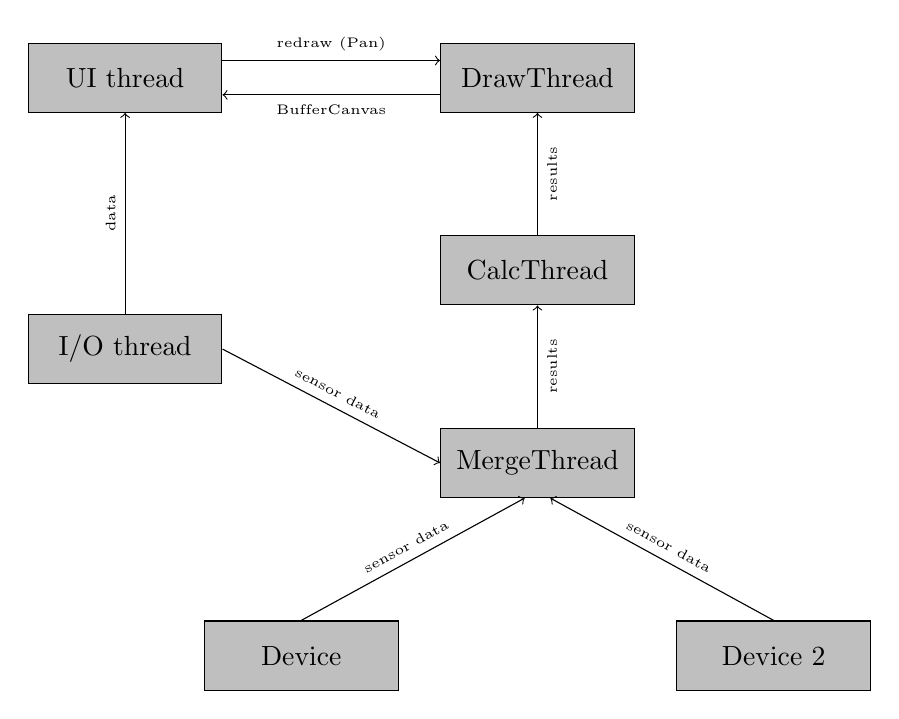
\begin{tikzpicture}
  \node(ui)[thread]{UI thread};

  \path(ui.east)+(4,0) node(draw)[thread]{DrawThread};
  \draw[->] (ui.10) -- (draw.170)
  node[midway, above, sloped, font=\tiny]{redraw (Pan)};
  \draw[->] (draw.190) -- (ui.350)
  node[midway, below, sloped, font=\tiny]{BufferCanvas};

  \path(draw.south)+(0,-2) node(calc)[thread]{CalcThread};
  \draw[->] (calc.north) -- (draw.south)
  node[midway, below, sloped, font=\tiny]{results};

  \path(calc.south)+(0,-2) node(merge)[thread]{MergeThread};
  \draw[->] (merge.north) -- (calc.south)
  node[midway, below, sloped, font=\tiny]{results};

  \path(merge.south)+(-3,-2) node(device1)[thread]{Device};
  \draw[->] (device1.north) -- (merge.250)
  node[midway, above, sloped, font=\tiny]{sensor data};

  \path(merge.south)+(3,-2) node(device2)[thread]{Device 2};
  \draw[->] (device2.north) -- (merge.290)
  node[midway, above, sloped, font=\tiny]{sensor data};

  \path(ui.south)+(0,-3) node(io)[thread]{I/O thread};
  \draw[->] (io.north) -- (ui.south)
  node[midway, above, sloped, font=\tiny]{data};
  \draw[->] (io.east) -- (merge.west)
  node[midway, above, sloped, font=\tiny]{sensor data};
\end{tikzpicture}

The UI thread is the main thread.  It starts the other threads and is
responsible for the UI event loop.  No other thread is allowed to
manipulate windows.  The UI thread has a timer which does regular
house keeping twice per second (\texttt{Pro\-cess\-Ti\-mer.cpp}).

The calculation thread (\texttt{Calcu\-la\-tion\-Thread.cpp},
\texttt{Glide\-Com\-pu\-ter*.cpp}) does all the expensive calculations
in background.  It gets data from the devices (through
\texttt{Merge\-Thread}) and forwards it together with calculation
results to the drawing thread and the main thread.

Each device has its own thread (\texttt{Serial\-Port.cpp}).  This is
needed because Windows CE does not support asynchronous COMM port I/O.
The thread is stopped during task declaration (which happens in the UI
thread).

When new data arrives on the serial port, the \texttt{Merge\-Thread}
gets notified, which will merge all sensor values into one data
structure.  It will then run cheap calculations, and forwards
everything to the \texttt{Calcu\-la\-tion\-Thread}.

With OpenGL, the map is rendered live without a buffer.  There is no
DrawThread.

On Android, the UI thread is not the main thread - the main thread is
implemented in Java, managed by Android itself.  The UI thread listens
for events which the Java part drops into the event queue
(\texttt{NativeView.java} and others).  The internal GPS does not need
a thread, it is implemented with Java callbacks.  For Bluetooth I/O,
there are two threads implemented in Java (\texttt{InputThread.java}
and \texttt{OutputThread.java}, managed by
\texttt{BluetoothHelper.java}).

\subsection{Locking}

Some data structures are rarely modified.  There is no lock for them.
For a modifications, all threads must be suspended.  Example:
waypoints, airspaces.

Other data structures are modified so often that correct locking would
be too much overhead.  Each thread and each instance has its own
copy.  The lock needs to be obtained only for making the private
copy.  The private copy can be used without locking.  Example:
\texttt{NMEA\_INFO}, \texttt{DERIVED\_INFO}.

There are objects which are too expensive to copy.  Normal locking
applies to them.  We have a template class called \texttt{Guard} to
enforce proper read/write locking.  Example: the task.


\section{Accessing Sensor Data}

Much of XCSoar deals with obtaining sensor data and visualising it.

Suppose you want to write a dialog that needs the current GPS
location, where do you get it?  The short and simple answer is: from
\verb|CommonInterface::Basic()| (the \texttt{InterfaceBlackboard}).
Example:

\begin{verbatim}
#include "Interface.hpp"

...
  const auto &basic = CommonInterface::Basic();
  if (basic.location_available)
    current_location = basic.location;
\end{verbatim}

This is true for the main thread (aka the ``user interface thread'').
Other threads must not use the \texttt{Interface.hpp} library, because
the \verb|InterfaceBlackboard| is not protected in any way.  It
contains copies of various data structures just for the main thread.

This is how sensor data moves inside XCSoar:

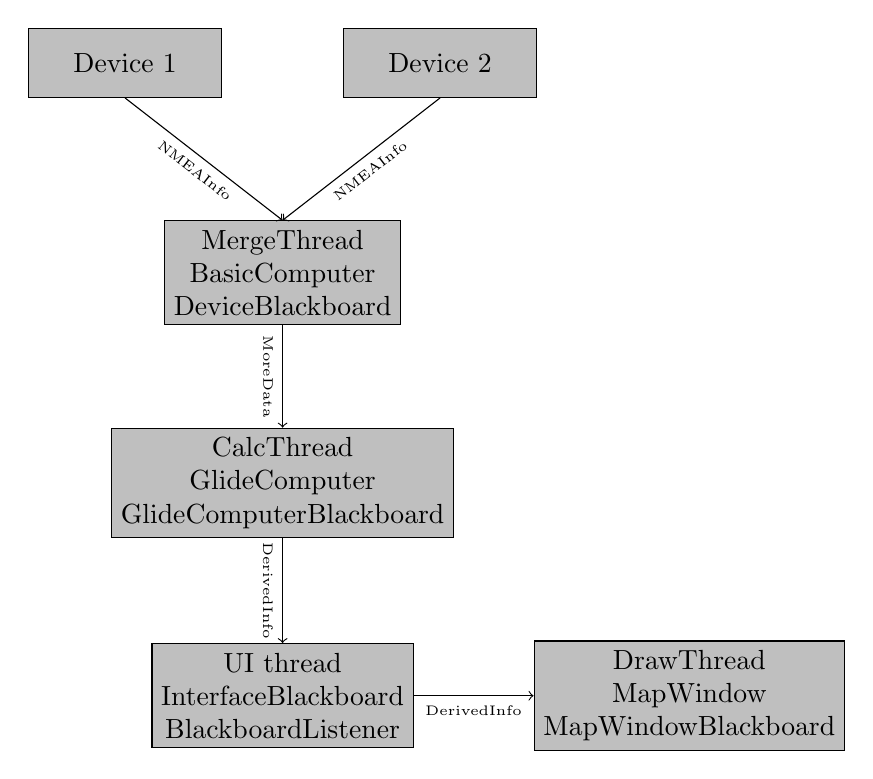
\begin{tikzpicture}
  \node(merge)[thread,align=center]{
    MergeThread\\
    BasicComputer\\
    DeviceBlackboard
  };

  \path(merge.north)+(-2,2) node(device1)[thread]{Device 1};
  \draw[->] (device1.south) -- (merge.north)
  node[midway, below, sloped, font=\tiny]{NMEAInfo};

  \path(merge.north)+(2,2) node(device2)[thread]{Device 2};
  \draw[->] (device2.south) -- (merge.north)
  node[midway, below, sloped, font=\tiny]{NMEAInfo};

  \path(merge.south)+(0,-2) node(calc)[thread,align=center]{
    CalcThread\\
    GlideComputer\\
    GlideComputerBlackboard
  };
  \draw[->] (merge.south) -- (calc.north)
  node[midway, below, sloped, font=\tiny]{MoreData};

  \path(calc.south)+(0,-2) node(ui)[thread,align=center]{
    UI thread\\
    InterfaceBlackboard\\
    BlackboardListener
  };
  \draw[->] (calc.south) -- (ui.north)
  node[midway, below, sloped, font=\tiny]{DerivedInfo};

  \path(ui.east)+(3.5,0) node(draw)[thread,align=center]{
    DrawThread\\
    MapWindow\\
    MapWindowBlackboard
  };
  \draw[->] (ui.east) -- (draw.west)
  node[midway, below, sloped, font=\tiny]{DerivedInfo};
\end{tikzpicture}

The device driver parses input received from its device into its own
\texttt{NMEAInfo} instance inside \texttt{DeviceBlackboard}
(i.e. \verb|per_device_data|).  Then it wakes up the
\texttt{MergeThread} to merge the new data into the central
\texttt{NMEAInfo} instance.  The \texttt{MergeThread} hosts the
\texttt{BasicComputer} which attempts to calculate missing data (for
example, derives vario from GPS altitude).

The \texttt{CalculationThread} wakes up and receives the
\texttt{MoreData} object from \texttt{DeviceBlackboard}.  Here,
expensive calculations are performed (\texttt{GlideComputer}: task
engine, airspace warnings, ...), resulting in a \texttt{DerivedInfo}
object.  The \texttt{CalculationThread} runs no more than twice per
second.

Finally, the UI thread wakes up and receives \texttt{MoreData} and
\texttt{DerivedInfo} via \texttt{DeviceBlackboard}.  This updates
InfoBoxes and other UI elements.  On Windows, the map is drawn in a
separate thread, so there's another layer.

Let's get back to the question: where do I get sensor data?  That
depends on who you are:

\begin{itemize}

\item you are the user interface: (InfoBoxes, dialogs, any Window
  callback): \texttt{InterfaceBlackboard} (see above).  To get
  notified on changes, register a \texttt{BlackboardListener} (and
  don't forget to unregister it).

\item you are the MapWindow: depends!  If you're being called from
  \texttt{OnPaintBuffer} (i.e. inside the \texttt{DrawThread}), you
  must use the \texttt{MapWindowBlackboard}, all others must use the
  \texttt{InterfaceBlackboard}.

\item you are a ``computer'' library: you will get the values as a
  parameter.  Don't try to use the \texttt{GlideComputerBlackboard}
  directly.

\item you are a device driver: implement the method
  \texttt{OnSensorUpdate} or \texttt{OnCalculatedUpdate} if you need
  to know values from other devices or calculation results.

\item everybody else may use the \texttt{DeviceBlackboard}, but be
  sure to lock it while using its data.

\end{itemize}


\chapter{The build system}\label{cha:build}

A big plain \texttt{Makefile} is used to control the XCSoar build.
GNU extensions are allowed.

This chapter describes the internals of our build system; for
instructions on compiling XCSoar, see chapter \ref{cha:compiling}.

\section{Linker parameters}

The following variables (or variable suffixes) appear in the
\texttt{Makefile} (conforming to \texttt{automake} conventions):

\begin{description}
\item[\texttt{LDFLAGS}] Linker flags, such as \texttt{-static} or
  \texttt{-Wl,...}, but not \texttt{-l}.
\item[\texttt{LDLIBS}] All \texttt{-l} flags, e.g. \texttt{-lGL}.
\item[\texttt{LDADD}] Path names of static libraries,
  e.g. \texttt{/usr/lib/libz.a}.
\end{description}

Search directories (\texttt{-L}) are technically linker ``flags'', but
they are allowed in \texttt{LDLIBS}, too.


\chapter{Developing}

\section{Debugging XCSoar}

The XCSoar source repository contains a module for the GNU debugger
(\texttt{gdb}).  It contains pretty-printers for various XCSoar types,
including \texttt{Angle}, \texttt{GeoPoint} and others.  These are
helpful when you print values in the debugger.  To use it, start the
debugging session and load the module:

\begin{verbatim}
$ gdb -ex "source tools/gdb.py" output/UNIX/xcsoar
(gdb) run
\end{verbatim}

The module will automatically convert fixed-point to floating point,
radian angles to degrees and more.  You can now do fancy stuff like:

\begin{verbatim}
(gdb) p basic.location
$1 = GeoPoint(7.93911242887 51.1470221074)
(gdb) p basic.date_time_utc
$2 = DateTime(2012/12/23 21:41:57)
(gdb) p basic.track
$3 = 55.2254197961
(gdb) p basic.external_wind
$4 = GeoVector::ZERO
(gdb) p current_leg.vector_remaining
$5 = GeoVector(267.899420345 107957.109724)
\end{verbatim}



%%%%%%%%%%%%%%%%%%%%%%%%%%%%%%%%%%%%%%%%%%%%%%%%%%%%%%%%%%%%%%%
\chapter{User interface guidelines}

\section{General}

\begin{itemize}
\item Minimise the number of colours, and re-use colour groups already defined.
\item Too much use of colour where it is not required serves only to reduce 
 the effectiveness of bright colours for important items.
\item High colour saturation elements should be reserved for high importance items
\item High contrast against background should be reserved for high importance items
\item Attempt to adopt colours that are intuitive based the function of the item
\item Minimise the clutter where possible --- readibility is essential for use 
 in flight
\item Use colours defined in \verb|Graphics| according to functional name, not 
 their actual colour.
\item Try to maintain consistent use of colours in all uses of that function, 
 such as dialogue graphics as well as map overlays and infoboxes.
\item Text should always be monochrome.
\end{itemize}

Use aviation conventions or adopt best aviation human factors
standards where possible, in particular:
\begin{itemize}
\item ICAO Internation Standards and Recommended Practices, Annex 4 to the 
 Convention on International Civil Aviation (Aeronautical Charts).
\item NASA Colour Usage recommendations and design guidelines: \verb|http://colorusage.arc.nasa.gov/|
\item DOT/FAA/AR-03/67 {\em Human Factors Considerations in the Design and 
 Evaluation of Electronic Flight Bags (EFBs)} \verb|http://www.volpe.dot.gov/hf/aviation/efb/docs/efb_version2.pdf|
\item FAA Human Factors Design Standards \verb|http://hf.tc.faa.gov/hfds/|.
\item DOT/FAA/AM-01/17 {\em Human Factors Design Guidelines for Multifunction Displays}
\end{itemize}

Check for performance with respect to colour blindness.
This site has a useful tool that can be used to convert screenshots
to how they would look to a person with common color blindness:
\verb|http://www.etre.com/tools/colourcheck/|.

{\bf For safety purposes, avoid use of elements that may encourage or require 
the user to stare at the screen continuously.}

{\bf For safety purposes, avoid user controls that have significant risk of 
producing unsafe results if misconfigured by the pilot.}

\subsection{General colour conventions}
Colour conventions generally in use throughout the program:
\begin{itemize}
\item Red for indicator of warning
\item Orange for indicator of caution
\item Green for positive indicator of safety
\item Blue for neutral indicator of safety
\end{itemize}

\subsection{Displayed data}
\begin{itemize}
\item Where data is invalid, indicate this by not presenting the data or
  showing dashes.
\item Present data in user-defined units.
\item Display numerical data with significant digits appropriate to the accuracy of the
  calculations, or its functional use by the pilot, whichever is lower.
\end{itemize}

\section{Dialogs and menu buttons}

\subsection{Colors}
Colour conventions in use are:
\begin{itemize}
\item Grey for buttons
\item Buttons and other widgets rendered with an evenly shaded border
\item Yellow for clicked items
\item Light blue for the key focused item
\item Medium blue for dialogue title bar
\item Text is black if the item is enabled
\item Text is greyed out (but still visible) if the item is disabled
\end{itemize}

\subsection{dialogue types and navigation buttons}
There are four types of dialogs in XCSoar, and the navigation 
buttons for each are different.  
Navigation buttons are the Close, OK, Cancel and Select buttons.
\begin{itemize}
\item Dialogs that modify and save data when the dialogue closes.

These shall usually have a Close button (no Cancel) and may have context specific 
function buttons
\item Dialogs that modify data where Cancel would be important for the user.

These shall have OK and Cancel buttons.  This may include dialogs with 
children dialogs where hitting Cancel from the parent dialogue cancels 
all the changes made in the children dialogs

\item Dialogs that have a list of values, one of which can be selected to 
 return to the parent dialogue.

These shall have Select and Cancel buttons
\item Dialogs that display information that cannot be modified.

These shall have a Close button
\end{itemize}

\subsection{dialogue button placement and size}
\begin{itemize}
\item The Close and Cancel buttons will never appear in the same dialogue and 
 are always located in the same place.  This location will be:

For portrait: lower right

For landscape: lower left
\item The Select button will be accompanied with a Cancel button.  The locations will be:

For portrait: Select in lower left, Cancel in lower right

For landscape: Cancel in lower left, Select immediately above it
\item Buttons will be 35 (scaled) pixels high
\item Buttons will be flush with the bottom of the screen and with the sides of 
 the screen and against each other (no margins)
\item In portrait, buttons will be 33% or 50% or 100% width of the screen
\item In landscape, buttons will be 65 to 80 (scaled) pixels wide, as wide as the 
 frame permits.  They will generally be a vertical row of buttons flush left of the screen
\item If text won't fit on a button, the buttons can be made larger consistently 
 for a screen, but this should be the exception because if it must contain that 
 much text consider using a different type of control.
\item Exceptions to all the dialogue concepts above are encouraged, but should be 
 mocked up and reviewed with the development community prior to implementing and 
 possibly documenting in the developers guide.
\end{itemize}

\subsection{Usability}
\begin{itemize}
\item Minimum size of buttons should be X by Y mm
\item Ensure all dialogs are navigable using cursor keys only
\item Ensure the focussed item is clearly identified.  The rectangle
  of the widget on the canvas may be drawn using the \verb|fill_focus| method
  of \verb|Canvas|.
\end{itemize}

\section{Main graphics}

\subsection{Colors}
Colour conventions in use, in order of priority, are:
\begin{itemize}
\item Aircraft black and white, for neutrality but clear identification
\item Traffic (FLARM) use alarm green, orange, and red.
\item Lift is vibrant green, sink is copper orange.
\item Aircraft navigation (route, best cruise track) is (ICAO) dark purple-blue
\item Task navigation lines and areas are (ICAO) magenta.
\item Updraft sources and other updraft derived data is sky blue.
\end{itemize}

(Todo) airspace alert colours

Map culture (topography) and terrain rendering should conform to ICAO
Annex 4 where appropriate.  Note that some modifications are
reasonable for electronic use given that Annex 4 deals with paper
charts.  Nevertheless, the colour conventions are useful to adopt as they are
likely to be intuitive and are designed for aviation use.

\subsection{Pen styles}

\begin{itemize}
\item Map culture should be rendered with a thin pen
\item Thicker pens used for important (e.g.\ task, navigational, airspace) lines
\item Dashed lines are used to increase perceptual priority
\end{itemize}

\subsection{Map overlays}
Elements on the map that are not part of the map layer, such as additional
informational widgets (final glide bar, wind, north arrow) should be rendered
so as to help those elements be visually separated from the map:

\begin{itemize}
\item Generally adopt higher contrast (higher colour saturation or darker shade) 
 than the background map layer elements.

\item For elements covering an area (non line), draw the entire element or a border
with a luminosity contrasting pen, of width \verb|IBLSCALE(1)|.

\item Consider whether the widget is required in all flying states and display modes.
if it does not serve a direct functional purpose in some states/modes, do not
render it.

\item Avoid locating widgets at the aircraft symbol (ownship symbol).
It is important to keep this area clear so the aircraft symbol can be easily found.

\end{itemize}

Elements that may be rendered over each other should be organised in order of
priority, particularly with alert warning items above caution items above non-alert items.

\section{Terminology}
\subsection{Glide Ratio}
'Glide ratio' is a non-specific term which can refer to the ratio of horizontal to 
vertical motion with reference to either the surrounding airmass or the ground.

To reduce confusion, ground-referenced glide ratios (eg distance travelled over 
ground vs altitude lost) should be referred to by the term 'glide ratio over 
ground' when space allows, or 'glide ratio' / 'GR'.

Air-referenced glide ratios (eg airspeed vs sink rate) should be specified as 
'lift/drag ratio' / 'L/D ratio' / 'LD'. The lift/drag ratio is numerically equal 
to the air-referenced glide ratio when flying at constant speed.

If usage spans both air-referenced and ground-referenced glide ratios, the 
non-specific term 'glide ratio' / 'GR' should be used. 'Lift/drag ratio' should 
never be used to refer to ground-referenced glide ratios.

\chapter{File formats}\label{cha:file_formats}

\section{Input Events}

\subsection{Introduction}

The Input System is actually a large number of things all bunched into one.

Primarily it is about giving the user control of what button does what
and when. There is a new concept called Input Mode - this is a the
mode the GUI is in for input. For example, you can click on the info
boxes and you are now in "infobox" mode. Clicking on the map is called
"default". But it doesn't stop there, you can create a new mode called
anything you like. This may not mean much - but wait till you combine
it with the rest of the features...

Input is not restricted to hardware buttons any more. You can map all
your hardware buttons (currently support for APP1 to APP6, Left,
Right, Up, Down and Enter, although I believe we can do some more) but
also any key code at all. This feature allows those with a built in
keyboard to use any key to map to any function in XCS. Where it comes
into real advantage is in external keyboards. There are a number of
bluetooth devices out there (eg: \url{http://shop.brando.com.hk/btgamepad.php}) 
which can map each of their
buttons to any key code - that key code can then be mapped to any
feature in XCS. You can then add to the hardware buttons the buttons
available to you on external devices. Other inputs (eg: Serial) are
also being looked at - and support is in the code for that extension.

We are striving towards a platform which is not only easier to use and
more intuitive, but also faster and easier to use in flight as
well. As such, another new feature as part of input is the concept of
Button Labels. Combined with the modes mentioned above, you can create
any arbitrary set of functions to map to any number of buttons. Think
about it like creating a tree, or a multiple level menu.

This produces two benefits that I know will be appreciated by people
with limited inputs. The first is that you can create menus, where by
you press one button to get to the next level (eg: pressing on APP1
brings up AutoZoom, Pan Mode, Full screen on the other buttons. Press
APP1 again and it goes to Terrain, Marker and Auto MacCready. Press
APP1 again and the menu is gone) - but more importantly for those with
touch screens and limited buttons, each of these labels can optionally
be assigned a key and you can touch the button area as if it was a
button.  This means that we can actually control on a touch screen
model the entire system without buttons - press an area of the screen
and the buttons pop up, click through - change options and more.

The combined features of labels, configurable buttons (including from
external hardware), hierarchical menus (for lack of a better name),
touch screen buttons has allowed us to configure XCS - without
recompile - for an enormous range of hardware, and personal
preference.  And all configurable as plane text, simple files. There
is no need for a file, the defaults internally will probably be a
combination of a 4 button bottom system with one button always shown
on screen for no/few button display.

The screen layout - location of the labels - is also totally
configurable - allowing us to vary the layout of buttons depending on
the type of organiser or desired look and feel.

There is a great unexpected benefit in the development of the input
system.

We can execute any number of events attached to an input with only 2
extra lines of code. This worked perfectly. So now we have a basic
macro system, allowing many more events to be attached to a single
input event.

But it doesn't stop there, this has lead to some more excellent
developments. The idea of Glide Computer Events things like "Maximum
Altitude Reached". Currently we play a sound effect for that. But you
may choose to play a sound, bring up a message box and write to the
log file.

One nice feature of XCS is the ability to change things such as Zoom
and North when Circling. Now you can do so much more. You could choose
to point North, Zoom to 1.0 (rather than a relative change), Turn on
Vario Sounds, Start a timer. When switching back to Cruise mode, you
can bring up the stats box for 30 seconds. The options are limited by
your imagination.

This is also contributing to a major reduction in complex code. We can
move out these complex tests into one centrally, easier to manage
system, reducing bugs and improving maintainability.

Another side benefits of these Macros is User Defined Flight
Modes. One idea was a button which switched to Zoom 1.0, Pan ON, Pan
Move to Next Waypoint. Basically the ability to jump and see the next
waypoint. And in the previous we can change the Input Mode to
"ViewWaypoint" - at which point you can redefine the same button to
switch back to your original settings.

The flexibility of this system comes with only one small price. We
can't provide an interface within XCS to fully customise all of these
near infinitely variable possibilities. However I believe that is
unnecessary anyway, you are not likely to change these sort of
features very often, and definitely not on the field. That does not
mean you can't, you can of course edit the plane(sic) text file to
change functions.

What this really means is that we can have people in the project
helping and contributing to the customising of XCS, without having to
change the code. This, especially on an open source project is
fantastic as it nicely separates the user interface changes from the
highly reliable part of the code. It also involves people who can
develop new interfaces and functions that are expert gliders but not
necessarily programmers.

For information on file formats see Common/Data/Input/template.xci and
the web site documentation.


\subsection{Defaults and Files}

The file in the source Common/Data/input/template.xci is used to generate
automatically the C code necessary for the default configuration. However it is
in the exact same format as can be read in by XCS and therefore can be used
literally as a template for a more complicated file.

When you create your own file, you will need to select it as the Input File
within XCSoar Menu/Settings/Input Files, and then restart XCS.


\subsection{File format}

The file is plain text, with key=value pairs and a blank line to indicate
the end of a record.

\begin{verbatim}
mode=default
type=key
data=APP1
event=StatusMessage My favorite settings are done
event=ScreenModes full
event=Sounds on
event=Zoom 1.0
event=Pan off
label=My Prefs
location=1
\end{verbatim}

The record above demonstrates remapping the first hardware key on your
organiser to change Pan to off, Zoom to 1.0 Sounds on, ScreenModes
full, and then a status message to tell you it is done.

Lines are terminated by the stanard DOS newline which is CRLF (Carrage
Return then Line Feed). Records are terminated by an extra new line.

\subsection{Event order}

Until further work is done on processing, events are actually done in
reverse order - also known as RPN. This is because the events work on
the stack principle. Each one is pushed onto the stack for execution,
and then executed by popping back off the stack. This has reduced
complexity of the code base.

When writing input events, have a look where you put the StatusMessage
and make sure that it is at the top, not the bottom (if you have one).

\subsection{Event list}

{\footnotesize
\begin{tabular}{l|p{7cm}}
\emph{Event} & \emph{Description} \\

\hline

\texttt{ChangeInfoBoxType} \emph{C} & Possible arguments: next,
previous. \\

\hline

\texttt{MainMenu} & \\

\hline

\texttt{MarkLocation} & Mark a location. \\

\hline

\texttt{Mode} \emph{M} & Set the screen mode. \\

\hline

\texttt{Pan} \emph{P} & Control pan mode.  Possible arguments: on
(enable pan), off (disable pan), up, down, left, right \\

\hline

\texttt{PlaySound} \emph{S} & Play the specified sound. \\

\hline

\texttt{SelectInfoBox} \emph{S} & Possible
arguments: next, previous. \\

\hline

\texttt{SnailTrail} \emph{S} & Change snail trail setting.  Possible
arguments: off, short, long, show. \\

\hline

\texttt{ScreenModes} \emph{M} & Set the screen mode.  Possible
arguments: normal, auxilary, toggleauxiliary, full, togglefull,
toggle. \\

\hline

\texttt{Sounds} \emph{S} & Change vario sounds.  Possible arguments:
toggle, on, off, show. \\

\hline

\texttt{StatusMessage} \emph{M} & Display the specified status
message. \\

\hline

\texttt{Zoom} \emph{Z} & Everything about zoom of map.  Possible
arguments: auto toogle, auto on, auto off, auto show, in, out, +, ++,
-, --. \\

\end{tabular}}

\subsection{Modes}

XCSoar now has the concept of Modes. These are an arbitrary
string that associates with where and what XCS is doing.

Note: a mode entry in a record can have multiple entries by using a space
between eg: "infobox menu1 menu2"

\subsubsection{List of known modes}

\begin{description}
\item[\texttt{default}] Really map mode, where you mostly are
\item[\texttt{infobox}] An info box has been selected on the scrreen
\item[\texttt{*}] Any other arbitrary string
\end{description}

Mode precedence has been tricky, so instead of solving the problem 
it is being worked around. XCS will choose to set a global variable 
to specify what mode it thinks it is in. This can then be used by the
input code to decide what to do. This mode could get out of sink
with the real world, and careful checking will be required, but at
this stage it seems like the only sensible option.

The code will review first if an entry exists in the current mode, and 
then in the default mode. This allows you to do one of the following
example: Define a default action for button "A" to be "Zoom In" but
make that button increase Bugs value in infobox mode only. You can do
this by making an "default" and a "infobox" entry. You can also put an entry
in for Button "A" for every mode and have complete control.

Special Modes - eg: the level of a menu (Think File vs Edit, vs Tools vs Help)

have special modes, such as
the level of the menu you are at. You press one button, then another
set become available (like pressing menu and seeing Settings etc). This
will be very useful in non-touch screen models. The menu configuration
can then be read from this same file and configured, allowing any
number of levels and any number of combinations.

The only hard part is what mode to go back to. We need a 
"Calculate Live Mode" function - which can be called to calculate the
real live mode (eg: finalglide vs curse) rather than the temporary
mode such as Menu, Special Menu Level, Warning etc.

The label and location values are examples of what can be done here
to allow input button labels to be displayed. What needs to be 
considered is a simple way of mapping the locations and the size.
In some models it may be that buttons are 4 across the top of the
screen, where as others it is 3 or 2 or even 6. So both size and
location needs to be considered.

The label itself will go through gettext to allow language
translations.

\subsection{Keys}

The key type can have the following possible values:

\begin{description}
\item[\texttt{APP1-APP6}] Hardware key on pocket pc
\item[\texttt{F1-F12}] Standard function keys
\item[\texttt{LEFT, RIGHT, UP, DOWN, RETURN}] Mapped to arrow keys - joystick on
  organisers
\item[\texttt{A-Z, 0-9}] and other possible keyboard buttons (case is ignored)
\end{description}


XXX Review...
Input Types

Types:

hardware	These are the standard hardware buttons 
on normal organisers. Usually these are
APP1..6.

keyboard	Normal characters on the keyboard (a-z etc)

nmea		A sentence received via NMEA stream (either)

virtual		Virtual buttons are a new idea, allowing
multiple buttons to be created on screen.
These buttons can then be optionally mapped
to physical buttons or to a spot on the 
screen (probably transparent buttons over 
the map).

Modifiers

It is a long term goal of this project to allow modifiers for keys.
This could include one of the following possibilities:

\begin{itemize}
\item Combination presses (although not supported on many devices)
\item Double Click
\item Long Click
\end{itemize}

Modifiers such as the above will not be supported in the first release.

\begin{verb}
Functions/Events - what it does

AutoZoom		on, off, toggle 
FullScreen		on, off, toggle
SnailTrail 		on, off, long, toggle
VarioSound 		on, off
Marker 			optional text to add
MenuButton 		on, off, toggle
Menu			open, close, toggle
MenuEntry		task, b+b, abortresume, abore, resume, pressure
logger, settings, status, analysis, exit, cancel
NOTE: Some of the above may be separate functions
Settings		(each setting, bring up to that point)
Bugs			add, subtract, 0-100% (set value)
Ballast			add, subtract, 0-100% (set value)
Zoom			add, subtract, 0-nn (set value)
Wind			up, down, 0-nn (set value, left, right, "n","ne","e","se","s","sw","w","nw"...
MacCready		add, subtract, 0-nn (set value)
WaypointNext		"String" to specific waypoint
eg: WayPointNext "home"
WayPoint???		"reverse" - reverse, from last passed back to start (ie: from here to home)
"drop next" - drop the next
"restore" - restore all - from start of flight but 
XXX This needs more thought
flight 			"startstop", "start", "stop", "release"
Start/Stop of flight - Can be automatic, but pressing will override
automatic part.
release 		markse the point of release from tow
\end{verb}

\subsection{Glide Computer Events}

These are automatically triggered events. They work in exactly the
same way, but instead of the user pressing a key, the glide computer
triggers the events.

A simple example is moving from Cruise to Climb mode. We want to zoom
in, change our track up to north up and switch to full screen. You may
also choose to drop a marker with the words "entered thermal". The
choicese are up to your imaginations - the GCE (Glide Computer Events)
allow you to control what happens.

These are represented as "type=gce" and data=* - as listed below.

{\footnotesize
\begin{tabular}{l|p{5.6cm}}
\emph{Event} & \emph{Description} \\
\hline

\verb|COMMPORT_RESTART| & The comm port is restarted. \\

\hline

\verb|FLIGHTMODE_CLIMB| & The flight mode has switched to ``climb''. \\

\hline

\verb|FLIGHTMODE_CRUIS| & The flight mode has switched to ``cruise''. \\

\hline

\verb|FLIGHTMODE_FINALGLIDE| & The flight mode has switched to ``final
glide''. \\

\hline

\verb|GPS_CONNECTION_WAIT| & Waiting for the GPS connection. \\

\hline

\verb|GPS_FIX_WAIT| & Waiting for a valid GPS fix. \\

\hline

\verb|HEIGHT_MAX| & Maximum height reached for this trip. \\

\hline

\verb|LANDING| & You are at landing. \\

\hline

\verb|STARTUP_REAL| & First message - this happens at startup of the
real XCS. \\

\hline

\verb|STARTUP_SIMULATOR| & Startup first message. This happens during
simulator mode. \\

\hline

\verb|TAKEOFF| & You have taken off. \\

\end{tabular}}

\section{Topography layer description file}
Each line of the topography layer description file (topography.tpl) contains
a comma seperated list (CSV) of information needed for rendering of an
individual topography layer. Lines starting with '*' are ignored.
\begin{table}[ht]
\centering
\sffamily
\begin{tabular}{@{}lll@{}}
\toprule
\addlinespace
Column name&Data type&Valid range\\
%\midrule
\cmidrule(r){1-1}\cmidrule(lr){2-2}\cmidrule(l){3-3}
filename&string&\\
range&double&-\\
icon&string&\\
label index&-&-\\
color (red component)&int&0-255\\
color (green component)&int&0-255\\
color (blue component)&int&0-255\\
pen width&int&0-31\\
label range&double&-\\
important label range&double&-\\
%\addlinespace
\bottomrule
\end{tabular}
\caption{Topography file format}
\label{tab:topography-file-format}
\end{table}

\begin{description}
\item[filename] The filename of the Topography layer within the container file.
\item[icon] XCSoar v6.5 and earlier, used only for town icons (219). From XCSoar v6.6, the name of the icon to display. Optional.
\item[range] A threshold zoom level. All layer elements will not be drawn
below this threshold.
\item[pen width] Lines contained within this layer are drawn with pen width.
\item[label range] A threshold zoom level. Labels contained in the layer file
will not be rendered below this threshold.
\item[important label range] A threshold zoom level. Labels contained
in the layer file will be rendered in standard style below this threshold.
\end{description}
\subsection{Point Features}
From XCSoar v6.6, a user can put an optional string into the icon column in topology.tpl in the .XCM file (e.g.)
\begin{itemize}
\item SpotHeight,5,\texttt{mountain\_top},1,64,64,64,1,5,
\item Mast,10,\texttt{obstacle},,,,,1,10,
\end{itemize}
This can be used for Shapefiles containing point features or polygons or linestrings, but is probably only useful for point features.

The icon of the corresponding image and optional label will be displayed. In the first example, 
the "mountain\_top" icon and a label will be displayed for each point in the SpotHeight shapefile. My
SpotHeight Shapefile has been generated with the point elevation in feet as the label value). For the second example, only "obstacle" icons 
(no labels) will be displayed for points in the Mast Shapefile..

Icon names are detected in TopographyStore.cpp. Names must be given in lowercase. If the icon name given is unknown, or no icon name is given, then icons are not displayed for that Shapefile.


Names correspond to images which have been linked into XCSoar, although
it is envisaged that in future these will be names of icon files. Available icon names are:
\begin{itemize}
\item mountain\_top \includegraphics[angle=0,width=8pt,keepaspectratio='true']{icons/map_mountain_top.pdf}
\item bridge \includegraphics[angle=0,width=8pt,keepaspectratio='true']{icons/map_bridge.pdf}
\item tunnel \includegraphics[angle=0,width=8pt,keepaspectratio='true']{icons/map_tunnel.pdf}
\item tower \includegraphics[angle=0,width=8pt,keepaspectratio='true']{icons/map_tower.pdf}
\item power\_plant \includegraphics[angle=0,width=8pt,keepaspectratio='true']{icons/map_power_plant.pdf}
\item obstacle \includegraphics[angle=0,width=8pt,keepaspectratio='true']{icons/map_obstacle.pdf}
\item mountain\_pass \includegraphics[angle=0,width=8pt,keepaspectratio='true']{icons/map_pass.pdf}
\item weather\_station \includegraphics[angle=0,width=8pt,keepaspectratio='true']{icons/map_weather_station.pdf}
\item thermal\_hotspot
\item town
\item mark \includegraphics[angle=0,width=8pt,keepaspectratio='true']{icons/map_flag.pdf}
\item turnpoint \includegraphics[angle=0,width=8pt,keepaspectratio='true']{icons/map_turnpoint.pdf}
\item small
\item cruise \includegraphics[angle=0,width=8pt,keepaspectratio='true']{icons/mode_cruise.pdf}
\item terrainwarning
\item logger
\item loggeroff
\item target
\item teammate\_pos
\item airspacei
\item traffic\_safe
\item traffic\_warning
\item traffic\_alarm
\item taskturnpoint
\item marginal \includegraphics[angle=0,width=8pt,keepaspectratio='true']{icons/winpilot_marginal.pdf}
\item landable \includegraphics[angle=0,width=8pt,keepaspectratio='true']{icons/winpilot_landable.pdf}
\item reachable \includegraphics[angle=0,width=8pt,keepaspectratio='true']{icons/winpilot_reachable.pdf}
\item airport\_reachable \includegraphics[angle=0,width=8pt,keepaspectratio='true']{icons/alt_reachable_airport.pdf}
\item airport\_unreachable \includegraphics[angle=0,width=8pt,keepaspectratio='true']{icons/alt_landable_airport.pdf}
\item airport\_marginal \includegraphics[angle=0,width=8pt,keepaspectratio='true']{icons/alt_marginal_airport.pdf}
\item airport\_unreachable2 \includegraphics[angle=0,width=8pt,keepaspectratio='true']{icons/alt2_landable_airport.pdf}
\item airport\_marginal2 \includegraphics[angle=0,width=8pt,keepaspectratio='true']{icons/alt2_marginal_airport.pdf}
\item outfield\_unreachable2 \includegraphics[angle=0,width=8pt,keepaspectratio='true']{icons/alt2_landable_field.pdf}
\item outfield\_marginal2 \includegraphics[angle=0,width=8pt,keepaspectratio='true']{icons/alt2_marginal_field.pdf}
\item outfield\_reachable \includegraphics[angle=0,width=8pt,keepaspectratio='true']{icons/alt_reachable_field.pdf}
\item outfield\_unreachable \includegraphics[angle=0,width=8pt,keepaspectratio='true']{icons/alt_landable_field.pdf}
\item outfield\_marginal \includegraphics[angle=0,width=8pt,keepaspectratio='true']{icons/alt_marginal_field.pdf}
\end{itemize}
\subsection{Adding new Icons}
At the moment, adding new icons requires a rebuild of the XCSoar application.It is envisaged that, in future, 
this process won't be required... users will include icon files in their .XCM map container files, and refer to them 
by name. However, that has not yet been implemented. 

To add your own images to the list of icons:
\begin{enumerate}
\item Create a .svg file for the icon (e.g. mast.svg) and copy into \texttt{xcsoar/Data/icons}. For Android, the name must be lowercase.
\item Insert two (for normal and high-res) lines into \texttt{xcsoar/Data/XCSoar.rc},  (e.g.)
\begin{verbatim}
BITMAP\_ICON(IDB\_MAST, "mast")
BITMAP\_ICON(IDB\_MAST\_HD, "mast\_160")
\end{verbatim}
\item Insert two lines into \texttt{xcsoar/src/resource.h} (e.g.)
\begin{verbatim}
\#define IDB\_MAST                        500
\#define IDB\_MAST\_HD                    5500
\end{verbatim}
\item Add a corresponding line into the \texttt{icon\_list} table in \texttt{xcsoar/src/Topography/TopographyStore.cpp}
\begin{verbatim}
  {"mast", IDB\_MAST},
\end{verbatim}
\item Make XCSoar
\end{enumerate} 
After this, a line can be added in \texttt{topology.tpl} to connect the icon to the Shapefile using the icon name. (e.g.)
\begin{verbatim}
Mast,10,mast,,,,,1,10,
\end{verbatim}

Note that unless these changes are merged into the main XCSoar repository, then only your specific build of XCSoar will be able to 
display your icon image.



%%%%%%%%%%%%%%%%%%%%%%%%%%%%%%%%%%%%%%%%%%%%%%%%%%%
\appendix

\chapter{GNU General Public License}\label{cha:gnu-general-public}

\begin{center}
{\large GNU General Public License}



Deutsche Übersetzung der Version 2, Juni 1991


{\sc Copyright © 1989, 1991 Free Software Foundation, Inc.\\
51 Franklin St, Fifth Floor, Boston, MA 02110, USA}
\end{center}

\vspace{0.75em}
Es ist {\sl jedermann} gestattet, diese Lizenzurkunde zu vervielfältigen und unveränderte Kopien zu verbreiten; Änderungen sind jedoch nicht erlaubt.


Diese Übersetzung ist kein rechtskräftiger Ersatz für die englischsprachige Originalversion! {\small (welche im Anhang beigefügt ist)}

\vspace{1em}

{\bf Vorwort}


{\small

Die meisten Softwarelizenzen sind daraufhin entworfen worden, Ihnen die Freiheit zu \textit{nehmen}, die Software weiterzugeben und zu verändern. Im Gegensatz dazu soll Ihnen die GNU General Public License, die Allgemeine Öffentliche GNU-Lizenz, ebendiese Freiheit garantieren. Sie soll sicherstellen, daß die Software für alle Benutzer frei ist. Diese Lizenz gilt für den Großteil der von der Free Software Foundation herausgegebenen Software und für alle anderen Programme, deren Autoren ihr Werk dieser Lizenz unterstellt haben. Auch Sie können diese Möglichkeit der Lizenzierung für Ihre Programme anwenden. (Ein anderer Teil der Software der Free Software Foundation unterliegt stattdessen der GNU Lesser General Public License, der Kleineren Allgemeinen Öffentlichen GNU-Lizenz.)

Die Bezeichnung „freie“ Software bezieht sich auf Freiheit, nicht auf den Preis. Unsere Lizenzen sollen Ihnen die Freiheit garantieren, Kopien freier Software zu verbreiten (und etwas für diesen Service zu berechnen, wenn Sie möchten), die Möglichkeit, die Software im Quelltext zu erhalten oder den Quelltext auf Wunsch zu bekommen. Die Lizenzen sollen garantieren, daß Sie die Software ändern oder Teile davon in neuen freien Programmen verwenden dürfen – und daß Sie wissen, daß Sie dies alles tun dürfen.

Um Ihre Rechte zu schützen, müssen wir Einschränkungen machen, die es jedem verbieten, Ihnen diese Rechte zu verweigern oder Sie aufzufordern, auf diese Rechte zu verzichten. Aus diesen Einschränkungen folgen bestimmte Verantwortlichkeiten für Sie, wenn Sie Kopien der Software verbreiten oder sie verändern.

Beispielsweise müssen Sie den Empfängern alle Rechte gewähren, die Sie selbst haben, wenn Sie – kostenlos oder gegen Bezahlung – Kopien eines solchen Programms verbreiten. Sie müssen sicherstellen, daß auch die Empfänger den Quelltext erhalten bzw. erhalten können. Und Sie müssen ihnen diese Bedingungen zeigen, damit sie ihre Rechte kennen.

Wir schützen Ihre Rechte in zwei Schritten: 

(1) Wir stellen die Software unter ein Urheberrecht (Copyright), und 

(2) wir bieten Ihnen diese Lizenz an, die Ihnen das Recht gibt, die Software zu vervielfältigen, zu verbreiten und/oder zu verändern.

Um die Autoren und uns zu schützen, wollen wir darüberhinaus sicherstellen, daß jeder erfährt, daß für diese freie Software keinerlei Garantie besteht. Wenn die Software von jemand anderem modifiziert und weitergegeben wird, möchten wir, daß die Empfänger wissen, daß sie nicht das Original erhalten haben, damit irgendwelche von anderen verursachte Probleme nicht den Ruf des ursprünglichen Autors schädigen.

Schließlich und endlich ist jedes freie Programm permanent durch Software-Patente bedroht. Wir möchten die Gefahr ausschließen, daß Distributoren eines freien Programms individuell Patente lizensieren – mit dem Ergebnis, daß das Programm proprietär würde. Um dies zu verhindern, haben wir klargestellt, daß jedes Patent entweder für freie Benutzung durch jedermann lizenziert werden muß oder überhaupt nicht lizenziert werden darf.


Es folgen die genauen Bedingungen für die Vervielfältigung, Verbreitung und Bearbeitung:



{\it Allgemeine Öffentliche GNU-Lizenz}

Bedingungen für die Vervielfältigung, Verbreitung und Bearbeitung
\begin{enumerate}
  \item Diese Lizenz gilt für jedes Programm und jedes andere Werk, in dem ein entsprechender Vermerk des Copyright-Inhabers darauf hinweist, daß das Werk unter den Bestimmungen dieser General Public License verbreitet werden darf. Im folgenden wird jedes derartige Programm oder Werk als „das Programm“ bezeichnet; die Formulierung „auf dem Programm basierendes Werk“ bezeichnet das Programm sowie jegliche Bearbeitung des Programms im urheberrechtlichen Sinne, also ein Werk, welches das Programm, auch auszugsweise, sei es unverändert oder verändert und/oder in eine andere Sprache übersetzt, enthält. (Im folgenden wird die Übersetzung ohne Einschränkung als „Bearbeitung“ eingestuft.) Jeder Lizenznehmer wird im folgenden als „Sie“ angesprochen.

Andere Handlungen als Vervielfältigung, Verbreitung und Bearbeitung werden von dieser Lizenz nicht berührt; sie fallen nicht in ihren Anwendungsbereich. Der Vorgang der Ausführung des Programms wird nicht eingeschränkt, und die Ausgaben des Programms unterliegen dieser Lizenz nur, wenn der Inhalt ein auf dem Programm basierendes Werk darstellt (unabhängig davon, daß die Ausgabe durch die Ausführung des Programmes erfolgte). Ob dies zutrifft, hängt von den Funktionen des Programms ab.

\item Sie dürfen auf beliebigen Medien unveränderte Kopien des Quelltextes des Programms, wie sie ihn erhalten haben, anfertigen und verbreiten. Voraussetzung hierfür ist, daß Sie mit jeder Kopie einen entsprechenden Copyright-Vermerk sowie einen Haftungsausschluß veröffentlichen, alle Vermerke, die sich auf diese Lizenz und das Fehlen einer Garantie beziehen, unverändert lassen und desweiteren allen anderen Empfängern des Programms zusammen mit dem Programm eine Kopie dieser Lizenz zukommen lassen.

Sie dürfen für den physikalischen Vorgang des Zugänglichmachens einer Kopie eine Gebühr verlangen. Wenn Sie es wünschen, dürfen Sie auch gegen Entgelt eine Garantie für das Programm anbieten.

\item Sie dürfen Ihre Kopie(n) des Programms oder eines Teils davon verändern, wodurch ein auf dem Programm basierendes Werk entsteht; Sie dürfen derartige Bearbeitungen unter den Bestimmungen von Paragraph 1 vervielfältigen und verbreiten, vorausgesetzt, daß zusätzlich alle im folgenden genannten Bedingungen erfüllt werden:

    Sie müssen die veränderten Dateien mit einem auffälligen Vermerk versehen, der auf die von Ihnen vorgenommene Modifizierung und das Datum jeder Änderung hinweist.

    Sie müssen dafür sorgen, daß jede von Ihnen verbreitete oder veröffentlichte Arbeit, die ganz oder teilweise von dem Programm oder Teilen davon abgeleitet ist, Dritten gegenüber als Ganzes unter den Bedingungen dieser Lizenz ohne Lizenzgebühren zur Verfügung gestellt wird.

    Wenn das veränderte Programm normalerweise bei der Ausführung interaktiv Kommandos einliest, müssen Sie dafür sorgen, daß es, wenn es auf dem üblichsten Wege für solche interaktive Nutzung gestartet wird, eine Meldung ausgibt oder ausdruckt, die einen geeigneten Copyright-Vermerk enthält sowie einen Hinweis, daß es keine Gewährleistung gibt (oder anderenfalls, daß Sie Garantie leisten), und daß die Benutzer das Programm unter diesen Bedingungen weiter verbreiten dürfen. Auch muß der Benutzer darauf hingewiesen werden, wie er eine Kopie dieser Lizenz ansehen kann. (Ausnahme: Wenn das Programm selbst interaktiv arbeitet, aber normalerweise keine derartige Meldung ausgibt, muß Ihr auf dem Programm basierendes Werk auch keine solche Meldung ausgeben).

Diese Anforderungen gelten für das bearbeitete Werk als Ganzes. Wenn identifizierbare Teile des Werkes nicht von dem Programm abgeleitet sind und vernünftigerweise als unabhängige und eigenständige Werke für sich selbst zu betrachten sind, dann gelten diese Lizenz und ihre Bedingungen nicht für die betroffenen Teile, wenn Sie diese als eigenständige Werke weitergeben. Wenn Sie jedoch dieselben Abschnitte als Teil eines Ganzen weitergeben, das ein auf dem Programm basierendes Werk darstellt, dann muß die Weitergabe des Ganzen nach den Bedingungen dieser Lizenz erfolgen, deren Bedingungen für weitere Lizenznehmer somit auf das gesamte Ganze ausgedehnt werden – und somit auf jeden einzelnen Teil, unabhängig vom jeweiligen Autor.

Somit ist es nicht die Absicht dieses Abschnittes, Rechte für Werke in Anspruch zu nehmen oder Ihnen die Rechte für Werke streitig zu machen, die komplett von Ihnen geschrieben wurden; vielmehr ist es die Absicht, die Rechte zur Kontrolle der Verbreitung von Werken, die auf dem Programm basieren oder unter seiner auszugsweisen Verwendung zusammengestellt worden sind, auszuüben.

Ferner bringt auch das einfache Zusammenlegen eines anderen Werkes, das nicht auf dem Programm basiert, mit dem Programm oder einem auf dem Programm basierenden Werk auf ein- und demselben Speicher- oder Vertriebsmedium dieses andere Werk nicht in den Anwendungsbereich dieser Lizenz.

\item Sie dürfen das Programm (oder ein darauf basierendes Werk gemäß Paragraph 2) als Objectcode oder in ausführbarer Form unter den Bedingungen der Paragraphen 1 und 2 kopieren und weitergeben – vorausgesetzt, daß Sie außerdem eine der folgenden Leistungen erbringen:
\begin{itemize}
    \item[a] Liefern Sie das Programm zusammen mit dem vollständigen zugehörigen maschinenlesbaren Quelltext auf einem für den Datenaustausch üblichen Medium aus, wobei die Verteilung unter den Bedingungen der Paragraphen 1 und 2 erfolgen muß. Oder:
    \item[b]Liefern Sie das Programm zusammen mit einem mindestens drei Jahre lang gültigen schriftlichen Angebot aus, jedem Dritten eine vollständige maschinenlesbare Kopie des Quelltextes zur Verfügung zu stellen – zu nicht höheren Kosten als denen, die durch das physikalische Zugänglichmachen des Quelltextes anfallen –, wobei der Quelltext unter den Bedingungen der Paragraphen 1 und 2 auf einem für den Datenaustausch üblichen Medium weitergegeben wird. Oder:
    \item[c]Liefern Sie das Programm zusammen mit dem schriftlichen Angebot der Zurverfügungstellung des Quelltextes aus, das Sie selbst erhalten haben. (Diese Alternative ist nur für nicht-kommerzielle Verbreitung zulässig und nur, wenn Sie das Programm als Objectcode oder in ausführbarer Form mit einem entsprechenden Angebot gemäß Absatz b erhalten haben.)
\end{itemize}
Unter dem Quelltext eines Werkes wird diejenige Form des Werkes verstanden, die für Bearbeitungen vorzugsweise verwendet wird. Für ein ausführbares Programm bedeutet „der komplette Quelltext“: Der Quelltext aller im Programm enthaltenen Module einschließlich aller zugehörigen Modulschnittstellen-Definitionsdateien sowie der zur Compilation und Installation verwendeten Skripte. Als besondere Ausnahme jedoch braucht der verteilte Quelltext nichts von dem zu enthalten, was üblicherweise (entweder als Quelltext oder in binärer Form) zusammen mit den Hauptkomponenten des Betriebssystems (Kernel, Compiler usw.) geliefert wird, unter dem das Programm läuft – es sei denn, diese Komponente selbst gehört zum ausführbaren Programm.

Wenn die Verbreitung eines ausführbaren Programms oder von Objectcode dadurch erfolgt, daß der Kopierzugriff auf eine dafür vorgesehene Stelle gewährt wird, so gilt die Gewährung eines gleichwertigen Kopierzugriffs auf den Quelltext von derselben Stelle als Verbreitung des Quelltextes, auch wenn Dritte nicht dazu gezwungen sind, den Quelltext zusammen mit dem Objectcode zu kopieren.

\item Sie dürfen das Programm nicht vervielfältigen, verändern, weiter lizenzieren oder verbreiten, sofern es nicht durch diese Lizenz ausdrücklich gestattet ist. Jeder anderweitige Versuch der Vervielfältigung, Modifizierung, Weiterlizenzierung und Verbreitung ist nichtig und beendet automatisch Ihre Rechte unter dieser Lizenz. Jedoch werden die Lizenzen Dritter, die von Ihnen Kopien oder Rechte unter dieser Lizenz erhalten haben, nicht beendet, solange diese die Lizenz voll anerkennen und befolgen.

\item  Sie sind nicht verpflichtet, diese Lizenz anzunehmen, da Sie sie nicht unterzeichnet haben. Jedoch gibt Ihnen nichts anderes die Erlaubnis, das Programm oder von ihm abgeleitete Werke zu verändern oder zu verbreiten. Diese Handlungen sind gesetzlich verboten, wenn Sie diese Lizenz nicht anerkennen. Indem Sie das Programm (oder ein darauf basierendes Werk) verändern oder verbreiten, erklären Sie Ihr Einverständnis mit dieser Lizenz und mit allen ihren Bedingungen bezüglich der Vervielfältigung, Verbreitung und Veränderung des Programms oder eines darauf basierenden Werks.

\item  Jedesmal, wenn Sie das Programm (oder ein auf dem Programm basierendes Werk) weitergeben, erhält der Empfänger automatisch vom ursprünglichen Lizenzgeber die Lizenz, das Programm entsprechend den hier festgelegten Bestimmungen zu vervielfältigen, zu verbreiten und zu verändern. Sie dürfen keine weiteren Einschränkungen der Durchsetzung der hierin zugestandenen Rechte des Empfängers vornehmen. Sie sind nicht dafür verantwortlich, die Einhaltung dieser Lizenz durch Dritte durchzusetzen.

\item Sollten Ihnen infolge eines Gerichtsurteils, des Vorwurfs einer Patentverletzung oder aus einem anderen Grunde (nicht auf Patentfragen begrenzt) Bedingungen (durch Gerichtsbeschluß, Vergleich oder anderweitig) auferlegt werden, die den Bedingungen dieser Lizenz widersprechen, so befreien Sie diese Umstände nicht von den Bestimmungen dieser Lizenz. Wenn es Ihnen nicht möglich ist, das Programm unter gleichzeitiger Beachtung der Bedingungen in dieser Lizenz und Ihrer anderweitigen Verpflichtungen zu verbreiten, dann dürfen Sie als Folge das Programm überhaupt nicht verbreiten. Wenn zum Beispiel ein Patent nicht die gebührenfreie Weiterverbreitung des Programms durch diejenigen erlaubt, die das Programm direkt oder indirekt von Ihnen erhalten haben, dann besteht der einzige Weg, sowohl das Patentrecht als auch diese Lizenz zu befolgen, darin, ganz auf die Verbreitung des Programms zu verzichten.

Sollte sich ein Teil dieses Paragraphen als ungültig oder unter bestimmten Umständen nicht durchsetzbar erweisen, so soll dieser Paragraph seinem Sinne nach angewandt werden; im übrigen soll dieser Paragraph als Ganzes gelten.

Zweck dieses Paragraphen ist nicht, Sie dazu zu bringen, irgendwelche Patente oder andere Eigentumsansprüche zu verletzen oder die Gültigkeit solcher Ansprüche zu bestreiten; dieser Paragraph hat einzig den Zweck, die Integrität des Verbreitungssystems der freien Software zu schützen, das durch die Praxis öffentlicher Lizenzen verwirklicht wird. Viele Leute haben großzügige Beiträge zu dem großen Angebot der mit diesem System verbreiteten Software im Vertrauen auf die konsistente Anwendung dieses Systems geleistet; es liegt am Autor/Geber, zu entscheiden, ob er die Software mittels irgendeines anderen Systems verbreiten will; ein Lizenznehmer hat auf diese Entscheidung keinen Einfluß.

Dieser Paragraph ist dazu gedacht, deutlich klarzustellen, was als Konsequenz aus dem Rest dieser Lizenz betrachtet wird.

\item Wenn die Verbreitung und/oder die Benutzung des Programms in bestimmten Staaten entweder durch Patente oder durch urheberrechtlich geschützte Schnittstellen eingeschränkt ist, kann der Urheberrechtsinhaber, der das Programm unter diese Lizenz gestellt hat, eine explizite geographische Begrenzung der Verbreitung angeben, in der diese Staaten ausgeschlossen werden, so daß die Verbreitung nur innerhalb und zwischen den Staaten erlaubt ist, die nicht ausgeschlossen sind. In einem solchen Fall beinhaltet diese Lizenz die Beschränkung, als wäre sie in diesem Text niedergeschrieben.

\item Die Free Software Foundation kann von Zeit zu Zeit überarbeitete und/oder neue Versionen der General Public License veröffentlichen. Solche neuen Versionen werden vom Grundprinzip her der gegenwärtigen entsprechen, können aber im Detail abweichen, um neuen Problemen und Anforderungen gerecht zu werden.

Jede Version dieser Lizenz hat eine eindeutige Versionsnummer. Wenn in einem Programm angegeben wird, daß es dieser Lizenz in einer bestimmten Versionsnummer oder „jeder späteren Version“ (“any later version”) unterliegt, so haben Sie die Wahl, entweder den Bestimmungen der genannten Version zu folgen oder denen jeder beliebigen späteren Version, die von der Free Software Foundation veröffentlicht wurde. Wenn das Programm keine Versionsnummer angibt, können Sie eine beliebige Version wählen, die je von der Free Software Foundation veröffentlicht wurde.

\item Wenn Sie den Wunsch haben, Teile des Programms in anderen freien Programmen zu verwenden, deren Bedingungen für die Verbreitung anders sind, schreiben Sie an den Autor, um ihn um die Erlaubnis zu bitten. Für Software, die unter dem Copyright der Free Software Foundation steht, schreiben Sie an die Free Software Foundation; wir machen zu diesem Zweck gelegentlich Ausnahmen. Unsere Entscheidung wird von den beiden Zielen geleitet werden, zum einen den freien Status aller von unserer freien Software abgeleiteten Werke zu erhalten und zum anderen das gemeinschaftliche Nutzen und Wiederverwenden von Software im allgemeinen zu fördern.
Keine Gewährleistung
\end{enumerate}

{\sc
Da das Programm ohne jegliche Kosten lizenziert wird, besteht keinerlei Gewährleistung für das Programm, soweit dies gesetzlich zulässig ist. Sofern nicht anderweitig schriftlich bestätigt, stellen die Copyright-Inhaber und/oder Dritte das Programm so zur Verfügung, „wie es ist“, ohne irgendeine Gewährleistung, weder ausdrücklich noch implizit, einschließlich – aber nicht begrenzt auf – Marktreife oder Verwendbarkeit für einen bestimmten Zweck. Das volle Risiko bezüglich Qualität und Leistungsfähigkeit des Programms liegt bei Ihnen. Sollte sich das Programm als fehlerhaft herausstellen, liegen die Kosten für notwendigen Service, Reparatur oder Korrektur bei Ihnen.

In keinem Fall, außer wenn durch geltendes Recht gefordert oder schriftlich zugesichert, ist irgendein Copyright-Inhaber oder irgendein Dritter, der das Programm wie oben erlaubt modifiziert oder verbreitet hat, Ihnen gegenüber für irgendwelche Schäden haftbar, einschließlich jeglicher allgemeiner oder spezieller Schäden, Schäden durch Seiteneffekte (Nebenwirkungen) oder Folgeschäden, die aus der Benutzung des Programms oder der Unbenutzbarkeit des Programms folgen (einschließlich – aber nicht beschränkt auf – Datenverluste, fehlerhafte Verarbeitung von Daten, Verluste, die von Ihnen oder anderen getragen werden müssen, oder dem Unvermögen des Programms, mit irgendeinem anderen Programm zusammenzuarbeiten), selbst wenn ein Copyright-Inhaber oder Dritter über die Möglichkeit solcher Schäden unterrichtet worden war. 
}
}


\vspace{1cm}
Auf den folgenden Seiten im Anschluß das englische Original der General Public License: 
\newpage 

{\small
\begin{center}
		    {\large GNU GENERAL PUBLIC LICENSE}

		       Version 2, June 1991


 {\sc Copyright (C) 1989, 1991 Free Software Foundation, Inc.\\
 59 Temple Place, Suite 330, Boston, MA  02111-1307  USA}
\end{center}

\vspace{0.75em}

 Everyone is permitted to copy and distribute verbatim copies
 of this license document, but changing it is not allowed.


\vspace{0.75cm}

{\bf Preamble}

\vspace{0.5cm}

  The licenses for most software are designed to take away your
freedom to share and change it.  By contrast, the GNU General Public
License is intended to guarantee your freedom to share and change free
software--to make sure the software is free for all its users.  This
General Public License applies to most of the Free Software
Foundation's software and to any other program whose authors commit to
using it.  (Some other Free Software Foundation software is covered by
the GNU Library General Public License instead.)  You can apply it to
your programs, too.

  When we speak of free software, we are referring to freedom, not
price.  Our General Public Licenses are designed to make sure that you
have the freedom to distribute copies of free software (and charge for
this service if you wish), that you receive source code or can get it
if you want it, that you can change the software or use pieces of it
in new free programs; and that you know you can do these things.

  To protect your rights, we need to make restrictions that forbid
anyone to deny you these rights or to ask you to surrender the rights.
These restrictions translate to certain responsibilities for you if you
distribute copies of the software, or if you modify it.

  For example, if you distribute copies of such a program, whether
gratis or for a fee, you must give the recipients all the rights that
you have.  You must make sure that they, too, receive or can get the
source code.  And you must show them these terms so they know their
rights.

  We protect your rights with two steps: (1) copyright the software, and
(2) offer you this license which gives you legal permission to copy,
distribute and/or modify the software.

  Also, for each author's protection and ours, we want to make certain
that everyone understands that there is no warranty for this free
software.  If the software is modified by someone else and passed on, we
want its recipients to know that what they have is not the original, so
that any problems introduced by others will not reflect on the original
authors' reputations.

  Finally, any free program is threatened constantly by software
patents.  We wish to avoid the danger that redistributors of a free
program will individually obtain patent licenses, in effect making the
program proprietary.  To prevent this, we have made it clear that any
patent must be licensed for everyone's free use or not licensed at all.

  The precise terms and conditions for copying, distribution and
modification follow.

\begin{center}
		    GNU GENERAL PUBLIC LICENSE

   TERMS AND CONDITIONS FOR COPYING, DISTRIBUTION AND MODIFICATION
\end{center}

\begin{enumerate}
\item This License applies to any program or other work which contains
a notice placed by the copyright holder saying it may be distributed
under the terms of this General Public License.  The "Program", below,
refers to any such program or work, and a "work based on the Program"
means either the Program or any derivative work under copyright law:
that is to say, a work containing the Program or a portion of it,
either verbatim or with modifications and/or translated into another
language.  (Hereinafter, translation is included without limitation in
the term "modification".)  Each licensee is addressed as "you".

Activities other than copying, distribution and modification are not
covered by this License; they are outside its scope.  The act of
running the Program is not restricted, and the output from the Program
is covered only if its contents constitute a work based on the
Program (independent of having been made by running the Program).
Whether that is true depends on what the Program does.

\item You may copy and distribute verbatim copies of the Program's
source code as you receive it, in any medium, provided that you
conspicuously and appropriately publish on each copy an appropriate
copyright notice and disclaimer of warranty; keep intact all the
notices that refer to this License and to the absence of any warranty;
and give any other recipients of the Program a copy of this License
along with the Program.

You may charge a fee for the physical act of transferring a copy, and
you may at your option offer warranty protection in exchange for a fee.

\item You may modify your copy or copies of the Program or any portion
of it, thus forming a work based on the Program, and copy and
distribute such modifications or work under the terms of Section 1
above, provided that you also meet all of these conditions:

\begin{enumerate}
    \item You must cause the modified files to carry prominent notices
    stating that you changed the files and the date of any change.

    \item You must cause any work that you distribute or publish, that in
    whole or in part contains or is derived from the Program or any
    part thereof, to be licensed as a whole at no charge to all third
    parties under the terms of this License.

    \item If the modified program normally reads commands interactively
    when run, you must cause it, when started running for such
    interactive use in the most ordinary way, to print or display an
    announcement including an appropriate copyright notice and a
    notice that there is no warranty (or else, saying that you provide
    a warranty) and that users may redistribute the program under
    these conditions, and telling the user how to view a copy of this
    License.  (Exception: if the Program itself is interactive but
    does not normally print such an announcement, your work based on
    the Program is not required to print an announcement.)
\end{enumerate}

These requirements apply to the modified work as a whole.  If
identifiable sections of that work are not derived from the Program,
and can be reasonably considered independent and separate works in
themselves, then this License, and its terms, do not apply to those
sections when you distribute them as separate works.  But when you
distribute the same sections as part of a whole which is a work based
on the Program, the distribution of the whole must be on the terms of
this License, whose permissions for other licensees extend to the
entire whole, and thus to each and every part regardless of who wrote it.

Thus, it is not the intent of this section to claim rights or contest
your rights to work written entirely by you; rather, the intent is to
exercise the right to control the distribution of derivative or
collective works based on the Program.

In addition, mere aggregation of another work not based on the Program
with the Program (or with a work based on the Program) on a volume of
a storage or distribution medium does not bring the other work under
the scope of this License.

\item You may copy and distribute the Program (or a work based on it,
under Section 2) in object code or executable form under the terms of
Sections 1 and 2 above provided that you also do one of the following:

\begin{enumerate}
    \item Accompany it with the complete corresponding machine-readable
    source code, which must be distributed under the terms of Sections
    1 and 2 above on a medium customarily used for software interchange; or,

    \item Accompany it with a written offer, valid for at least three
    years, to give any third party, for a charge no more than your
    cost of physically performing source distribution, a complete
    machine-readable copy of the corresponding source code, to be
    distributed under the terms of Sections 1 and 2 above on a medium
    customarily used for software interchange; or,

    \item Accompany it with the information you received as to the offer
    to distribute corresponding source code.  (This alternative is
    allowed only for noncommercial distribution and only if you
    received the program in object code or executable form with such
    an offer, in accord with Subsection b above.)
\end{enumerate}

The source code for a work means the preferred form of the work for
making modifications to it.  For an executable work, complete source
code means all the source code for all modules it contains, plus any
associated interface definition files, plus the scripts used to
control compilation and installation of the executable.  However, as a
special exception, the source code distributed need not include
anything that is normally distributed (in either source or binary
form) with the major components (compiler, kernel, and so on) of the
operating system on which the executable runs, unless that component
itself accompanies the executable.

If distribution of executable or object code is made by offering
access to copy from a designated place, then offering equivalent
access to copy the source code from the same place counts as
distribution of the source code, even though third parties are not
compelled to copy the source along with the object code.

\item You may not copy, modify, sublicense, or distribute the Program
except as expressly provided under this License.  Any attempt
otherwise to copy, modify, sublicense or distribute the Program is
void, and will automatically terminate your rights under this License.
However, parties who have received copies, or rights, from you under
this License will not have their licenses terminated so long as such
parties remain in full compliance.

\item You are not required to accept this License, since you have not
signed it.  However, nothing else grants you permission to modify or
distribute the Program or its derivative works.  These actions are
prohibited by law if you do not accept this License.  Therefore, by
modifying or distributing the Program (or any work based on the
Program), you indicate your acceptance of this License to do so, and
all its terms and conditions for copying, distributing or modifying
the Program or works based on it.

\item Each time you redistribute the Program (or any work based on the
Program), the recipient automatically receives a license from the
original licensor to copy, distribute or modify the Program subject to
these terms and conditions.  You may not impose any further
restrictions on the recipients' exercise of the rights granted herein.
You are not responsible for enforcing compliance by third parties to
this License.

\item If, as a consequence of a court judgment or allegation of patent
infringement or for any other reason (not limited to patent issues),
conditions are imposed on you (whether by court order, agreement or
otherwise) that contradict the conditions of this License, they do not
excuse you from the conditions of this License.  If you cannot
distribute so as to satisfy simultaneously your obligations under this
License and any other pertinent obligations, then as a consequence you
may not distribute the Program at all.  For example, if a patent
license would not permit royalty-free redistribution of the Program by
all those who receive copies directly or indirectly through you, then
the only way you could satisfy both it and this License would be to
refrain entirely from distribution of the Program.

If any portion of this section is held invalid or unenforceable under
any particular circumstance, the balance of the section is intended to
apply and the section as a whole is intended to apply in other
circumstances.

It is not the purpose of this section to induce you to infringe any
patents or other property right claims or to contest validity of any
such claims; this section has the sole purpose of protecting the
integrity of the free software distribution system, which is
implemented by public license practices.  Many people have made
generous contributions to the wide range of software distributed
through that system in reliance on consistent application of that
system; it is up to the author/donor to decide if he or she is willing
to distribute software through any other system and a licensee cannot
impose that choice.

This section is intended to make thoroughly clear what is believed to
be a consequence of the rest of this License.

\item If the distribution and/or use of the Program is restricted in
certain countries either by patents or by copyrighted interfaces, the
original copyright holder who places the Program under this License
may add an explicit geographical distribution limitation excluding
those countries, so that distribution is permitted only in or among
countries not thus excluded.  In such case, this License incorporates
the limitation as if written in the body of this License.

\item The Free Software Foundation may publish revised and/or new versions
of the General Public License from time to time.  Such new versions will
be similar in spirit to the present version, but may differ in detail to
address new problems or concerns.

Each version is given a distinguishing version number.  If the Program
specifies a version number of this License which applies to it and "any
later version", you have the option of following the terms and conditions
either of that version or of any later version published by the Free
Software Foundation.  If the Program does not specify a version number of
this License, you may choose any version ever published by the Free Software
Foundation.

\item If you wish to incorporate parts of the Program into other free
programs whose distribution conditions are different, write to the author
to ask for permission.  For software which is copyrighted by the Free
Software Foundation, write to the Free Software Foundation; we sometimes
make exceptions for this.  Our decision will be guided by the two goals
of preserving the free status of all derivatives of our free software and
of promoting the sharing and reuse of software generally.

\end{enumerate}

\subsection*{No warranty}
{\sc 
 BECAUSE THE PROGRAM IS LICENSED FREE OF CHARGE, THERE IS NO WARRANTY
 FOR THE PROGRAM, TO THE EXTENT PERMITTED BY APPLICABLE LAW.  EXCEPT
 WHEN OTHERWISE STATED IN WRITING THE COPYRIGHT HOLDERS AND/OR OTHER
 PARTIES PROVIDE THE PROGRAM "AS IS" WITHOUT WARRANTY OF ANY KIND,
 EITHER EXPRESSED OR IMPLIED, INCLUDING, BUT NOT LIMITED TO, THE
 IMPLIED WARRANTIES OF MERCHANTABILITY AND FITNESS FOR A PARTICULAR
 PURPOSE.  THE ENTIRE RISK AS TO THE QUALITY AND PERFORMANCE OF THE
 PROGRAM IS WITH YOU.  SHOULD THE PROGRAM PROVE DEFECTIVE, YOU ASSUME
 THE COST OF ALL NECESSARY SERVICING, REPAIR OR CORRECTION.

 IN NO EVENT UNLESS REQUIRED BY APPLICABLE LAW OR AGREED TO IN WRITING
 WILL ANY COPYRIGHT HOLDER, OR ANY OTHER PARTY WHO MAY MODIFY AND/OR
 REDISTRIBUTE THE PROGRAM AS PERMITTED ABOVE, BE LIABLE TO YOU FOR
 DAMAGES, INCLUDING ANY GENERAL, SPECIAL, INCIDENTAL OR CONSEQUENTIAL
 DAMAGES ARISING OUT OF THE USE OR INABILITY TO USE THE PROGRAM
 (INCLUDING BUT NOT LIMITED TO LOSS OF DATA OR DATA BEING RENDERED
 INACCURATE OR LOSSES SUSTAINED BY YOU OR THIRD PARTIES OR A FAILURE
 OF THE PROGRAM TO OPERATE WITH ANY OTHER PROGRAMS), EVEN IF SUCH
 HOLDER OR OTHER PARTY HAS BEEN ADVISED OF THE POSSIBILITY OF SUCH
 DAMAGES.
}
}





\endinput

\end{document}
